\documentclass{article}
\usepackage{graphicx}
\usepackage{amsmath}
\usepackage{amssymb}
\usepackage[italicdiff]{physics}
\usepackage{enumerate}
\usepackage{microtype}
\DisableLigatures{encoding= *, family=*}
\usepackage{titlesec}
\usepackage{xfrac}
\setcounter{secnumdepth}{4}
\usepackage{xcolor}
\usepackage[bookmarks=false]{hyperref}
\usepackage{mathtools}
\usepackage{tikz} 
\newcommand*\fullcirc[1][0.3ex]{\tikz\fill (0,0) circle (#1);} 
\usepackage{bigints}
\hypersetup{
    colorlinks=true,
    linkcolor=[RGB]{59 108 209},
    urlcolor=[RGB]{59 108 209}
}
\urlstyle{same}

\titleformat{\paragraph}
{\normalfont\normalsize\bfseries}{\theparagraph}{1em}{}
\titlespacing*{\paragraph}
{0pt}{3.25ex plus 1ex minus .2ex}{1.5ex plus .2ex}

\title{Hydrocarbon}
\author{}
\date{}

\begin{document}
\maketitle

\section{Free Radical Reactions}

\subsection{Reactions Shown by Free Radical}
\begin{enumerate}[i.]
    \item \textbf{Combination} \\
          Joining of two radicals, $2^\circ, 1^\circ$ majorly show combination.
    \item \textbf{Disproportionation} \\
          In case of $3^\circ$ radical combination is not possible, hence disproportionation occurs.
\end{enumerate}

\subsection{Important facts about Free Radicals}
\begin{itemize}
    \item Incomplete octet, $1$ unpaired $e^-$
    \item Highly unstable
    \item Paramagnetic
    \item Can be stabilized by both EDG and EWG.
    \item Neither a Lewis base nor a Lewis acid.
    \item $sp^2$ hybridized.
    \item Trigonal Planer Geometry.
\end{itemize}
\pagebreak
\begin{center}
    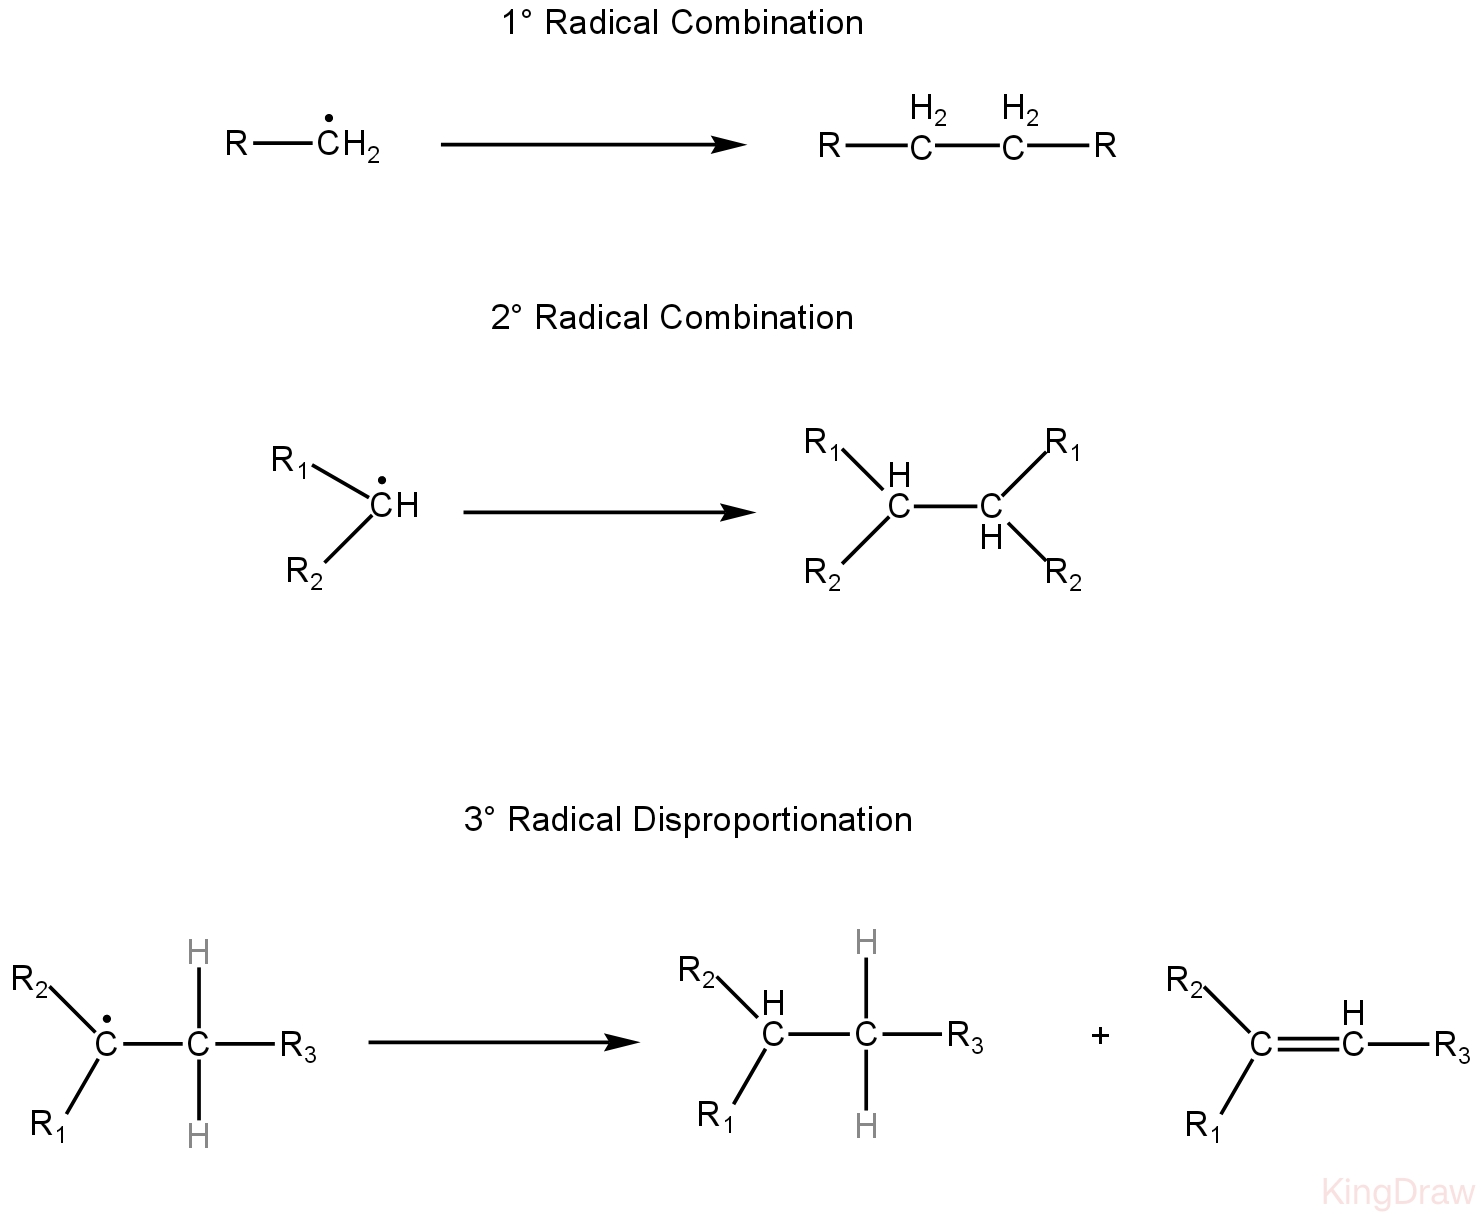
\includegraphics[scale=0.3]{FreeRadicalReaction(1)_1722161083701.JPEG}
\end{center}

\section{Wurtz Reaction}

\subsection{Reaction and Mechanism}
\begin{center}

    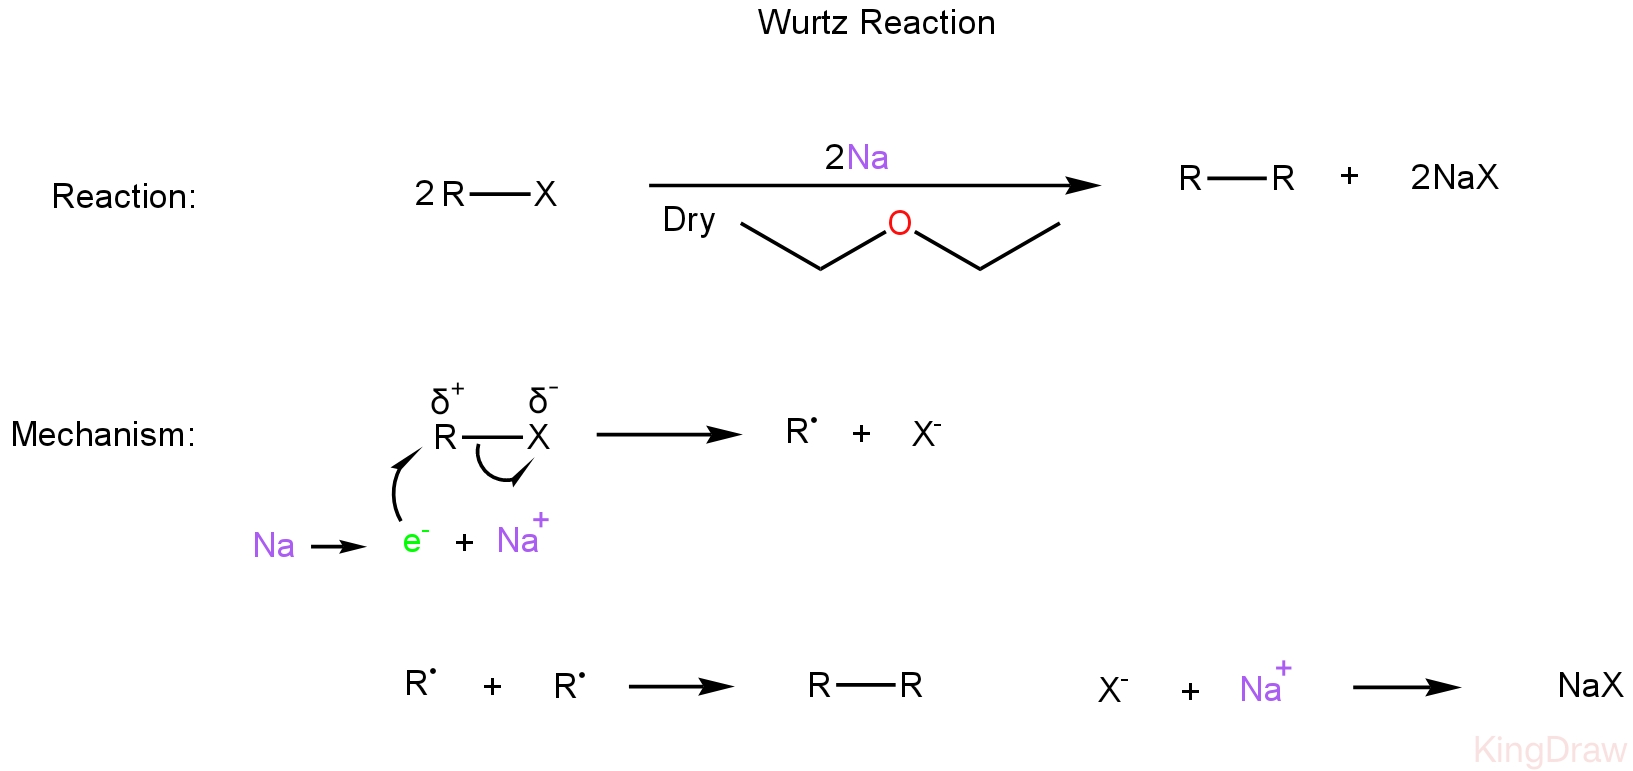
\includegraphics[scale=0.25]{WurtzReaction(1)_1722164749564.JPEG}
\end{center}

\subsection{Why dry $Et_{2}O$ is used instead of moisture?}
Water and Sodium metal react vigorously to form Sodium Hydroxide and evolve hydrogen gas, to avoid this reaction taking place dry environment is preferred.
\subsection{Why $Et_{2}O$ is used?}
$Et_{2}O$ is a PAS, hence it solvates only the cationic part (+).

\subsection{Reaction Observations}
\begin{enumerate}[i.]
    \item Free radical or $C^-$ obtained as intermediate.
    \item Breaking of $RX$ bond is RDS.
    \item $ROR$ for $RX$, $RI > RBr> RCl$
    \item $\textit{Stability of } R^\cdot \propto ROR $
    \item $RF$ doesn't react.
    \item $CH_{4}$ can never be obtained.
    \item Only symmetrical even number of $\prescript{12}{6}{C}$ obtained in very good yield.
    \item Unsymmetrical compound obtained in very poor yield.
\end{enumerate}

\section{Fittig Reaction}
\subsection{Reaction and Mechanism}
\begin{center}
    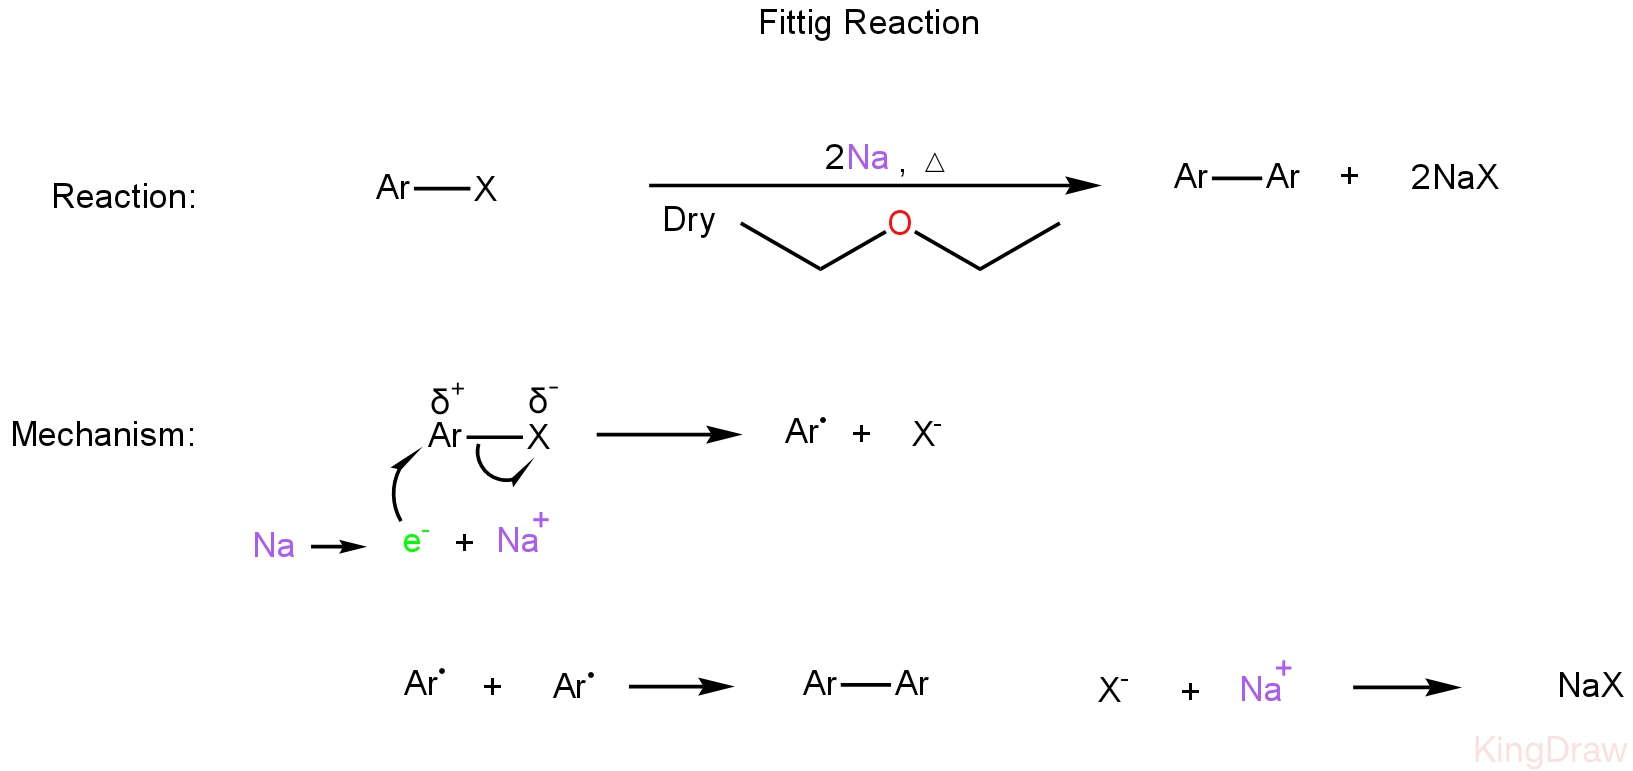
\includegraphics[scale=0.25]{Chem(1)_1722165285036.JPEG}
\end{center}

\section{Ulmann Reaction}
\subsection{Reaction and Mechanism}
\begin{center}
    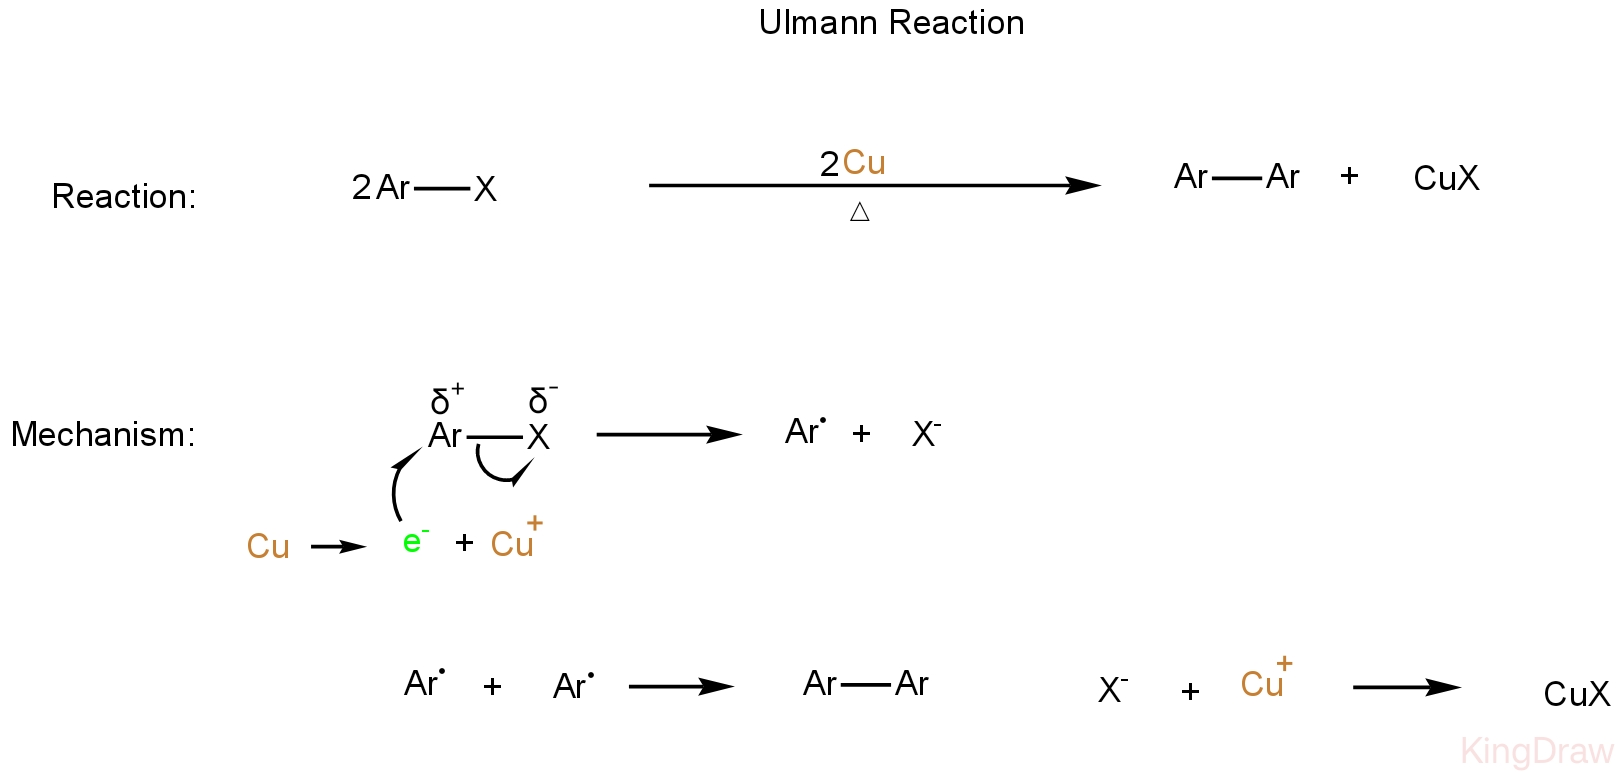
\includegraphics[scale=0.25]{UlmannReaction_1722165970453.JPEG}
\end{center}

\section{Frankland Reaction}
\subsection{Reaction and Mechanism}
\begin{center}
    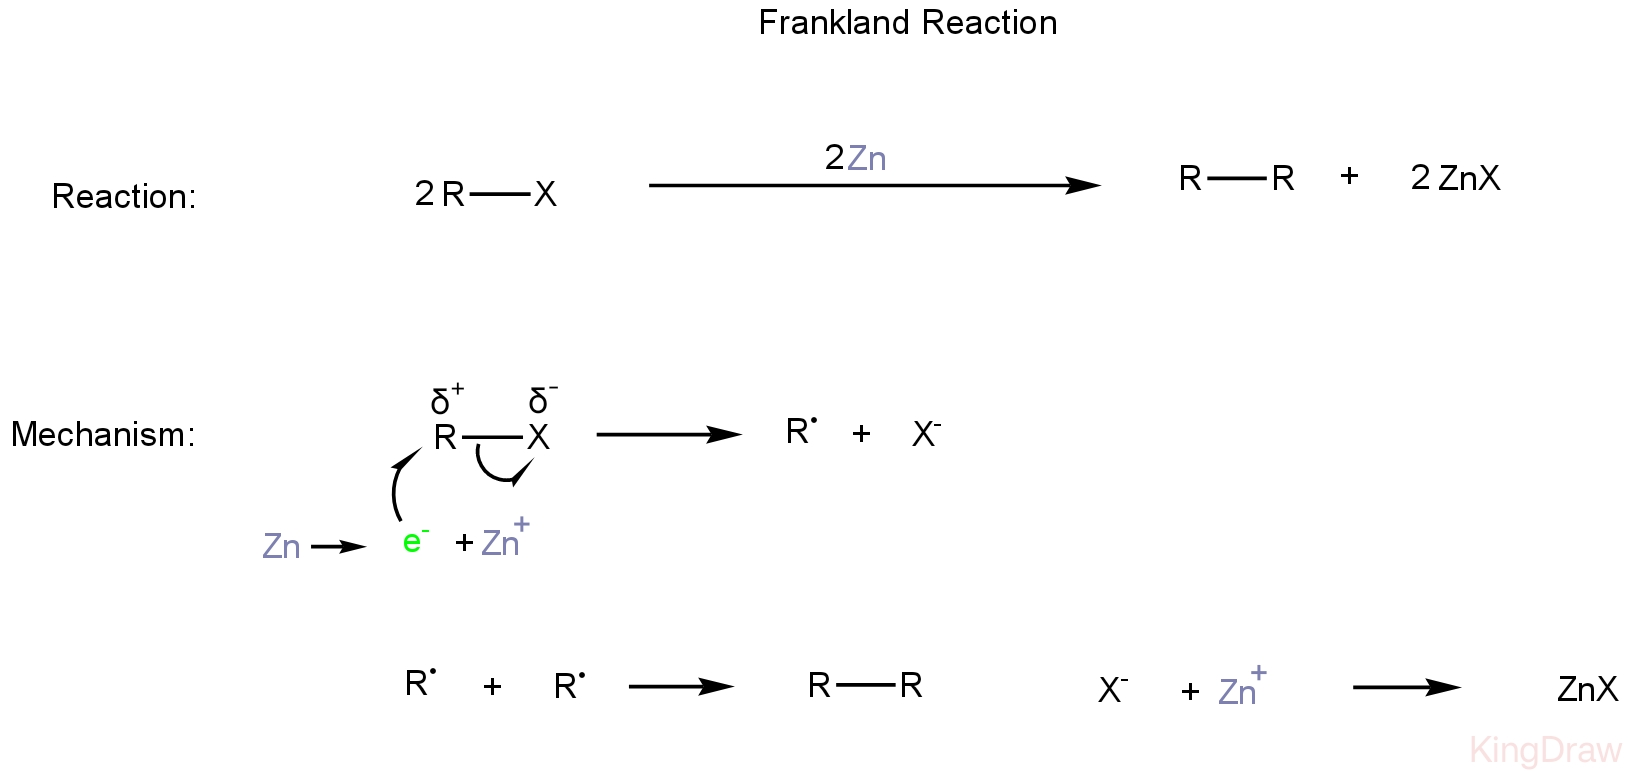
\includegraphics[scale=0.25]{FranklandReaction_1722166512574.JPEG}
\end{center}

\section{Wurtz-Fittig Reaction}
\subsection{Reaction and Mechanism}
\begin{center}
    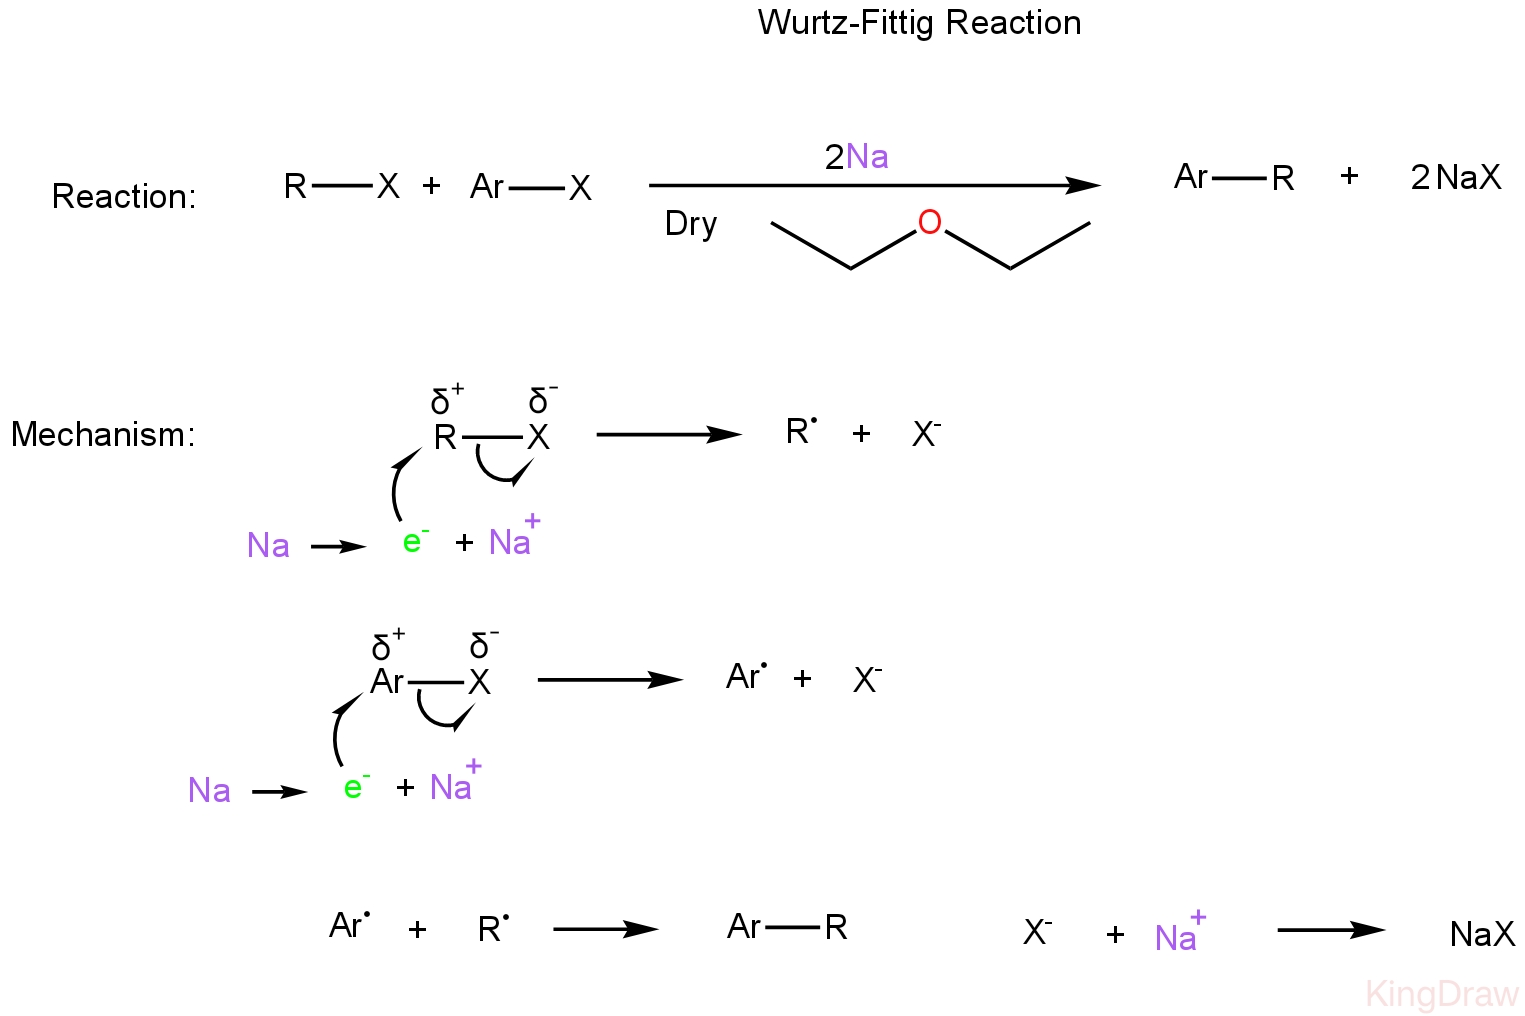
\includegraphics[scale=0.25]{WurtzFittigReaction_1722166913964.JPEG}
\end{center}

\section{Kolbe's Electrolysis}
\subsection{Reaction and Mechanism}
\begin{center}
    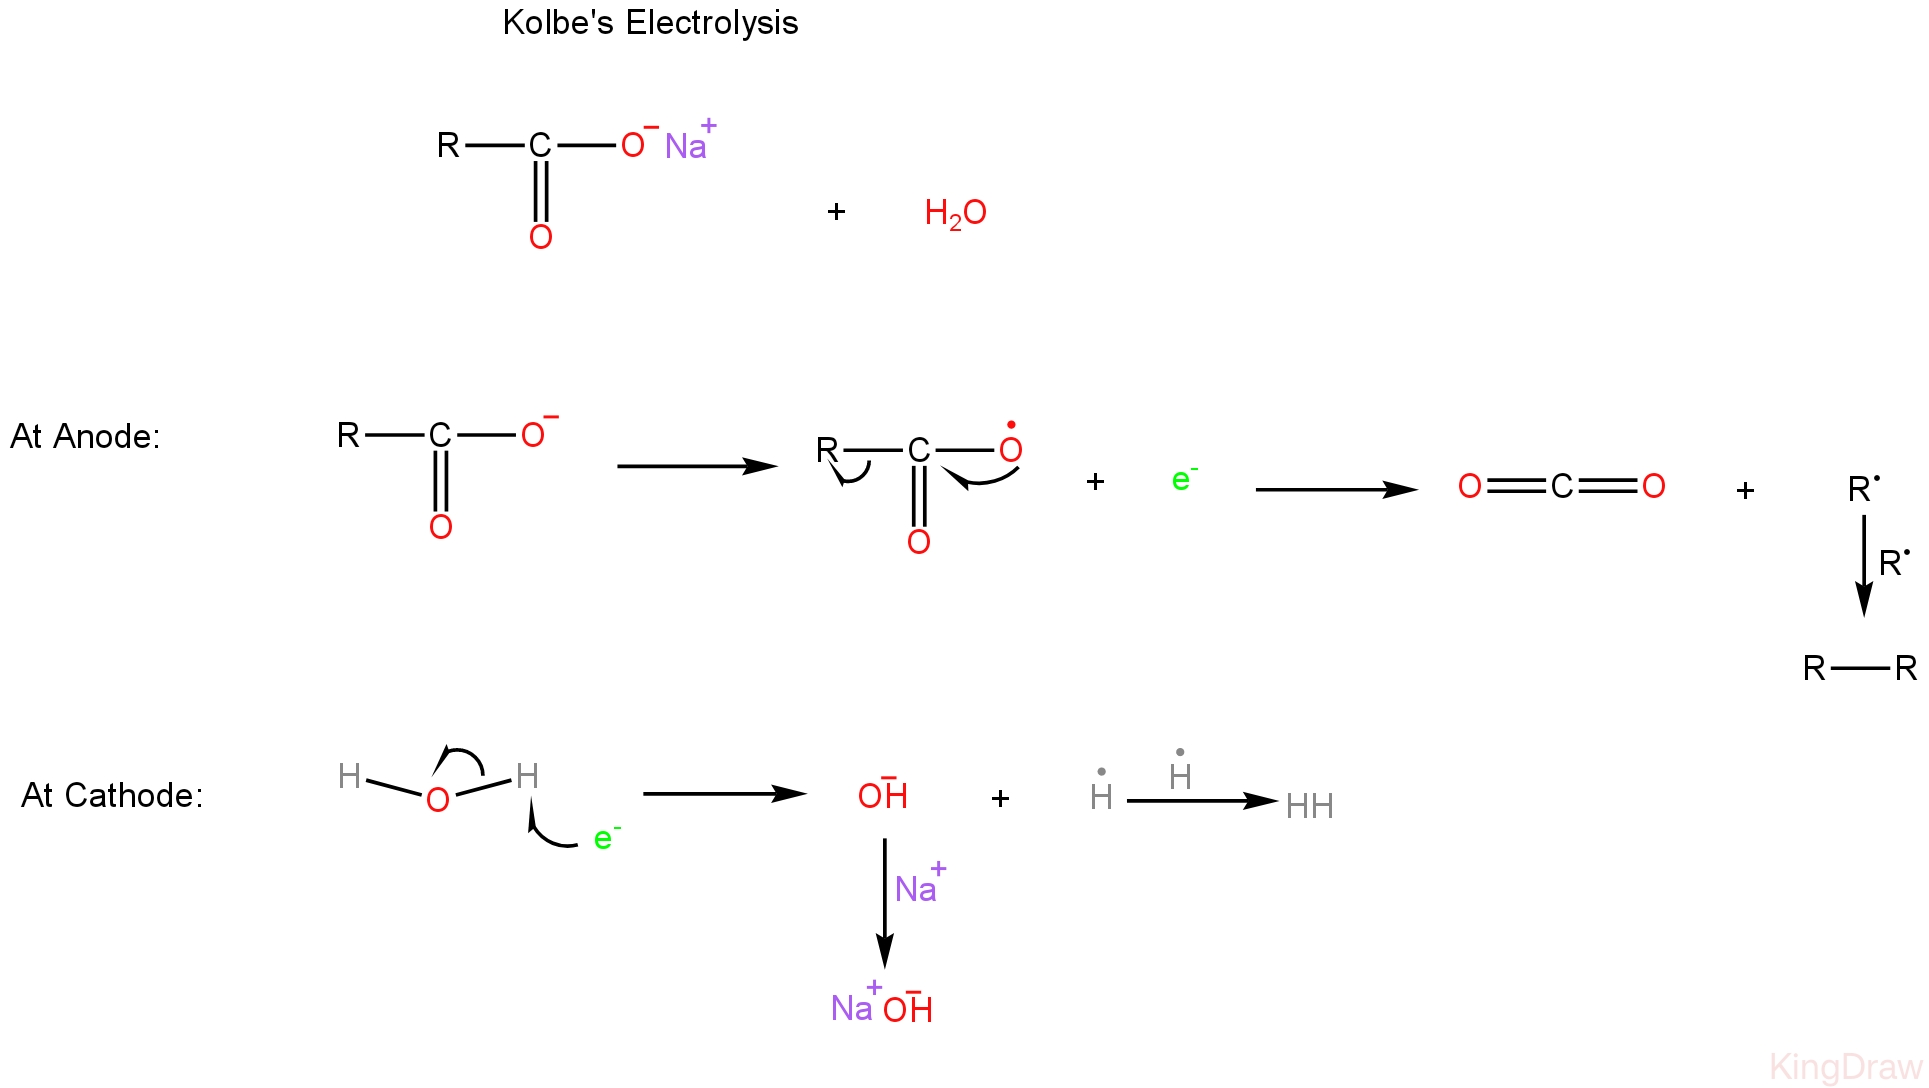
\includegraphics[scale=0.23]{Kolbe'sElectrolysis_1722168095985.JPEG}
\end{center}
\subsection{Reaction Observations}
\begin{enumerate}[i.]
    \item $C^{\fullcirc}$ obtained as intermediate.
    \item $pH$ of medium increases due to formation of $NaOH$.
    \item $CO_{2}$ obtained at anode and $H_{2}$ at cathode.
    \item $CH_{4}$ can never be obtained.
\end{enumerate}

\section{Formation of Grignard's Reagent}
\subsection{Reaction and Mechanism}
\begin{center}
    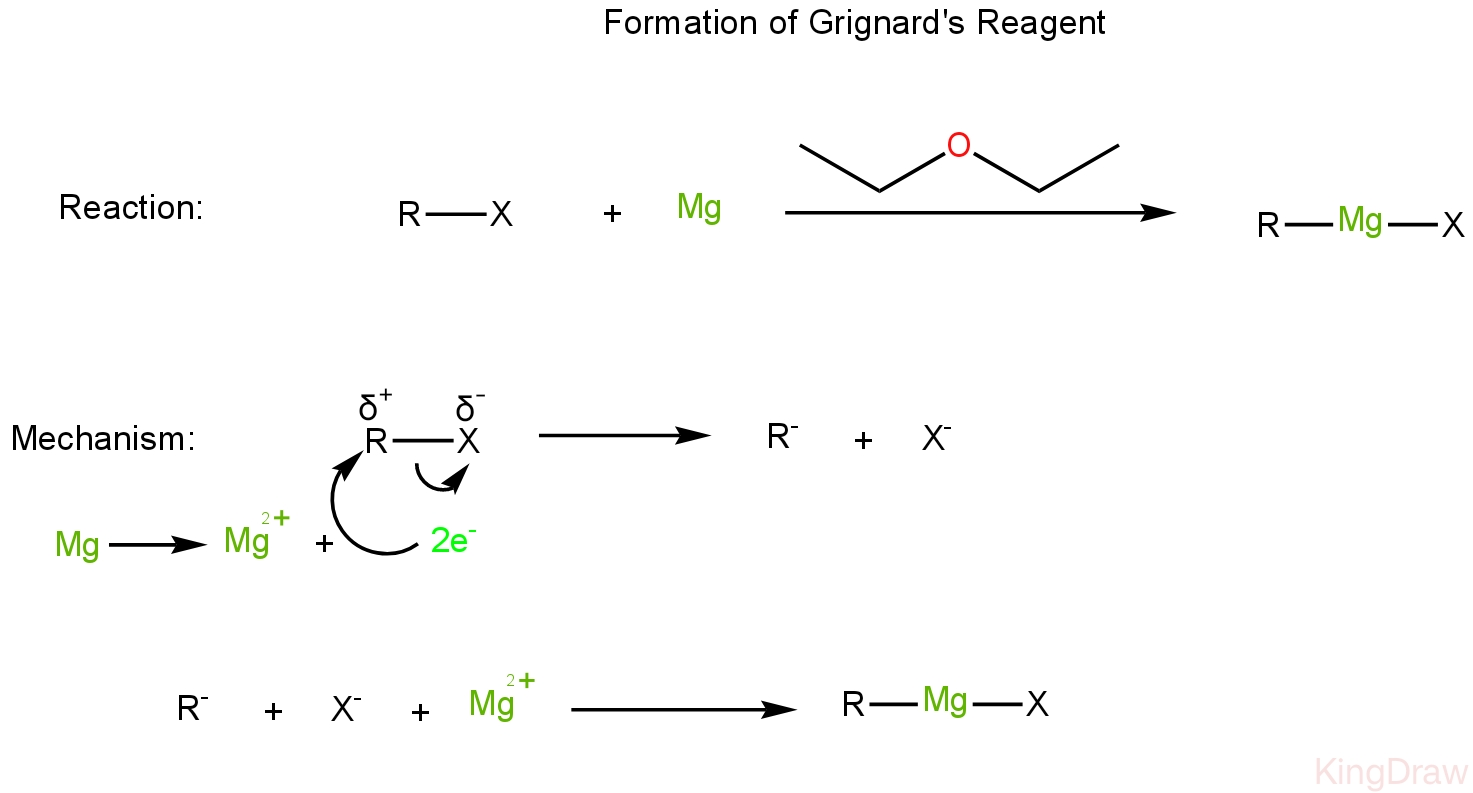
\includegraphics[scale=0.25]{FormationofGrignard'sReagent_1722171477216.JPEG}
\end{center}
\subsection{Reaction Observations}
\begin{enumerate}[i.]
    \item $C^-$ and $C^{\fullcirc}$ obtained as intermediate.
    \item $RMgX$ is also known as Organometallic Compound due to $\prescript{12}{6}{C}$ metal bond.
    \item $ROR$ for $RX$, $RI>RBr>RCl$
    \item Reaction doesn't occur in $RF$
    \item Dry $Et_{2}O$ or $THF$ is used as solvent.
\end{enumerate}

\section{Photo Halogenation}
\subsection{Reaction and Mechanism}
\begin{center}
    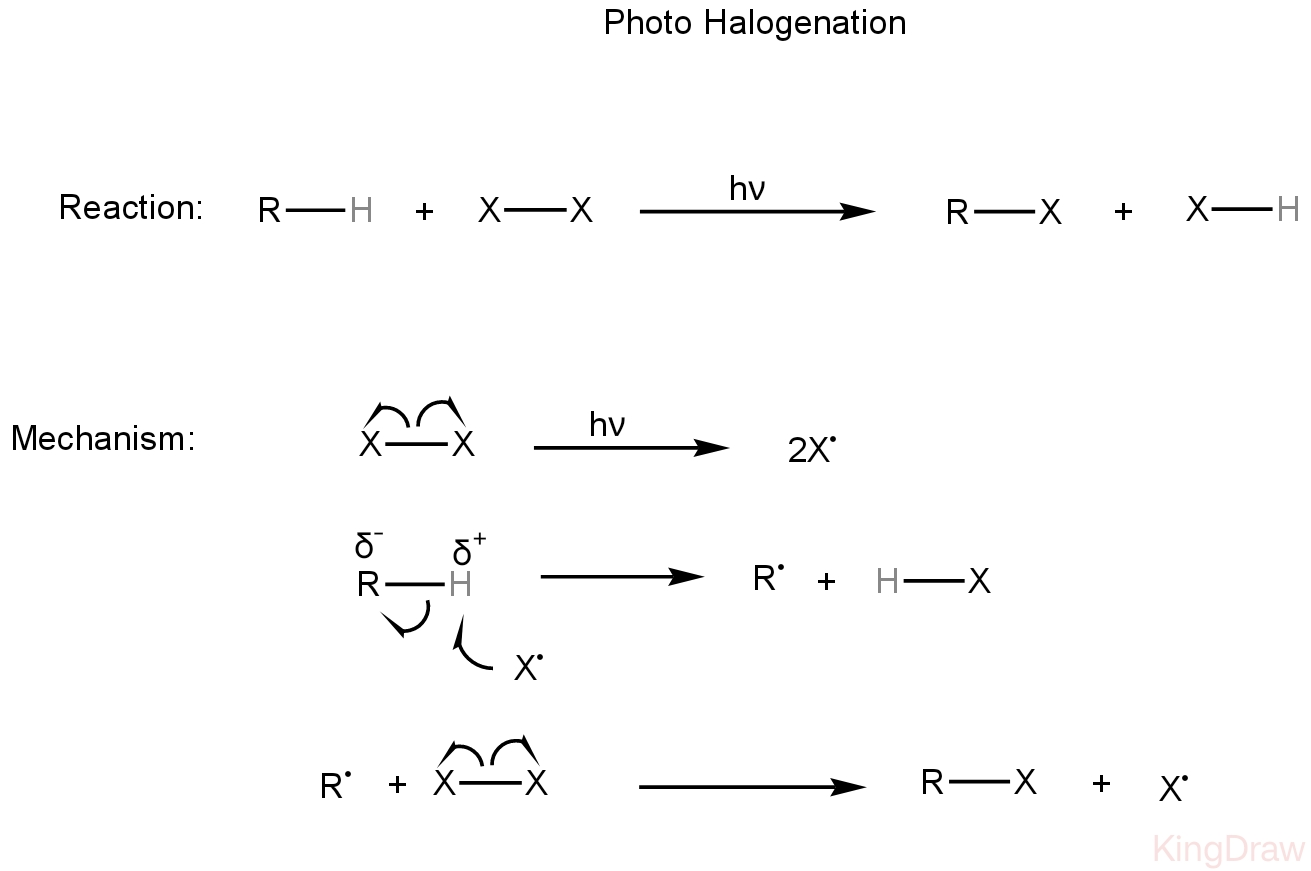
\includegraphics[scale=0.3]{PhotoHalogenanion_1722173018626.JPEG}
\end{center}

\subsection{Reaction Observations}
\begin{enumerate}[i.]
    \item $C^{\fullcirc}$ obtained as intermediate.
    \item Example of $C^{\fullcirc}$ substitution reaction.
    \item Kinetic isotopic effect is observed.
    \item Example of Oxidation reaction.
    \item Formation of $C^{\fullcirc}$ is RDS.
    \item $ROR \propto \textit{ Stability of } C^{\fullcirc}$
    \item $ROR$ for $X_{2}$, $F_{2}>Cl_{2}>Br_{2}>I_{2}$
\end{enumerate}

\section{Reed's Reaction}
\subsection{Reaction and Mechanism}
\begin{center}
    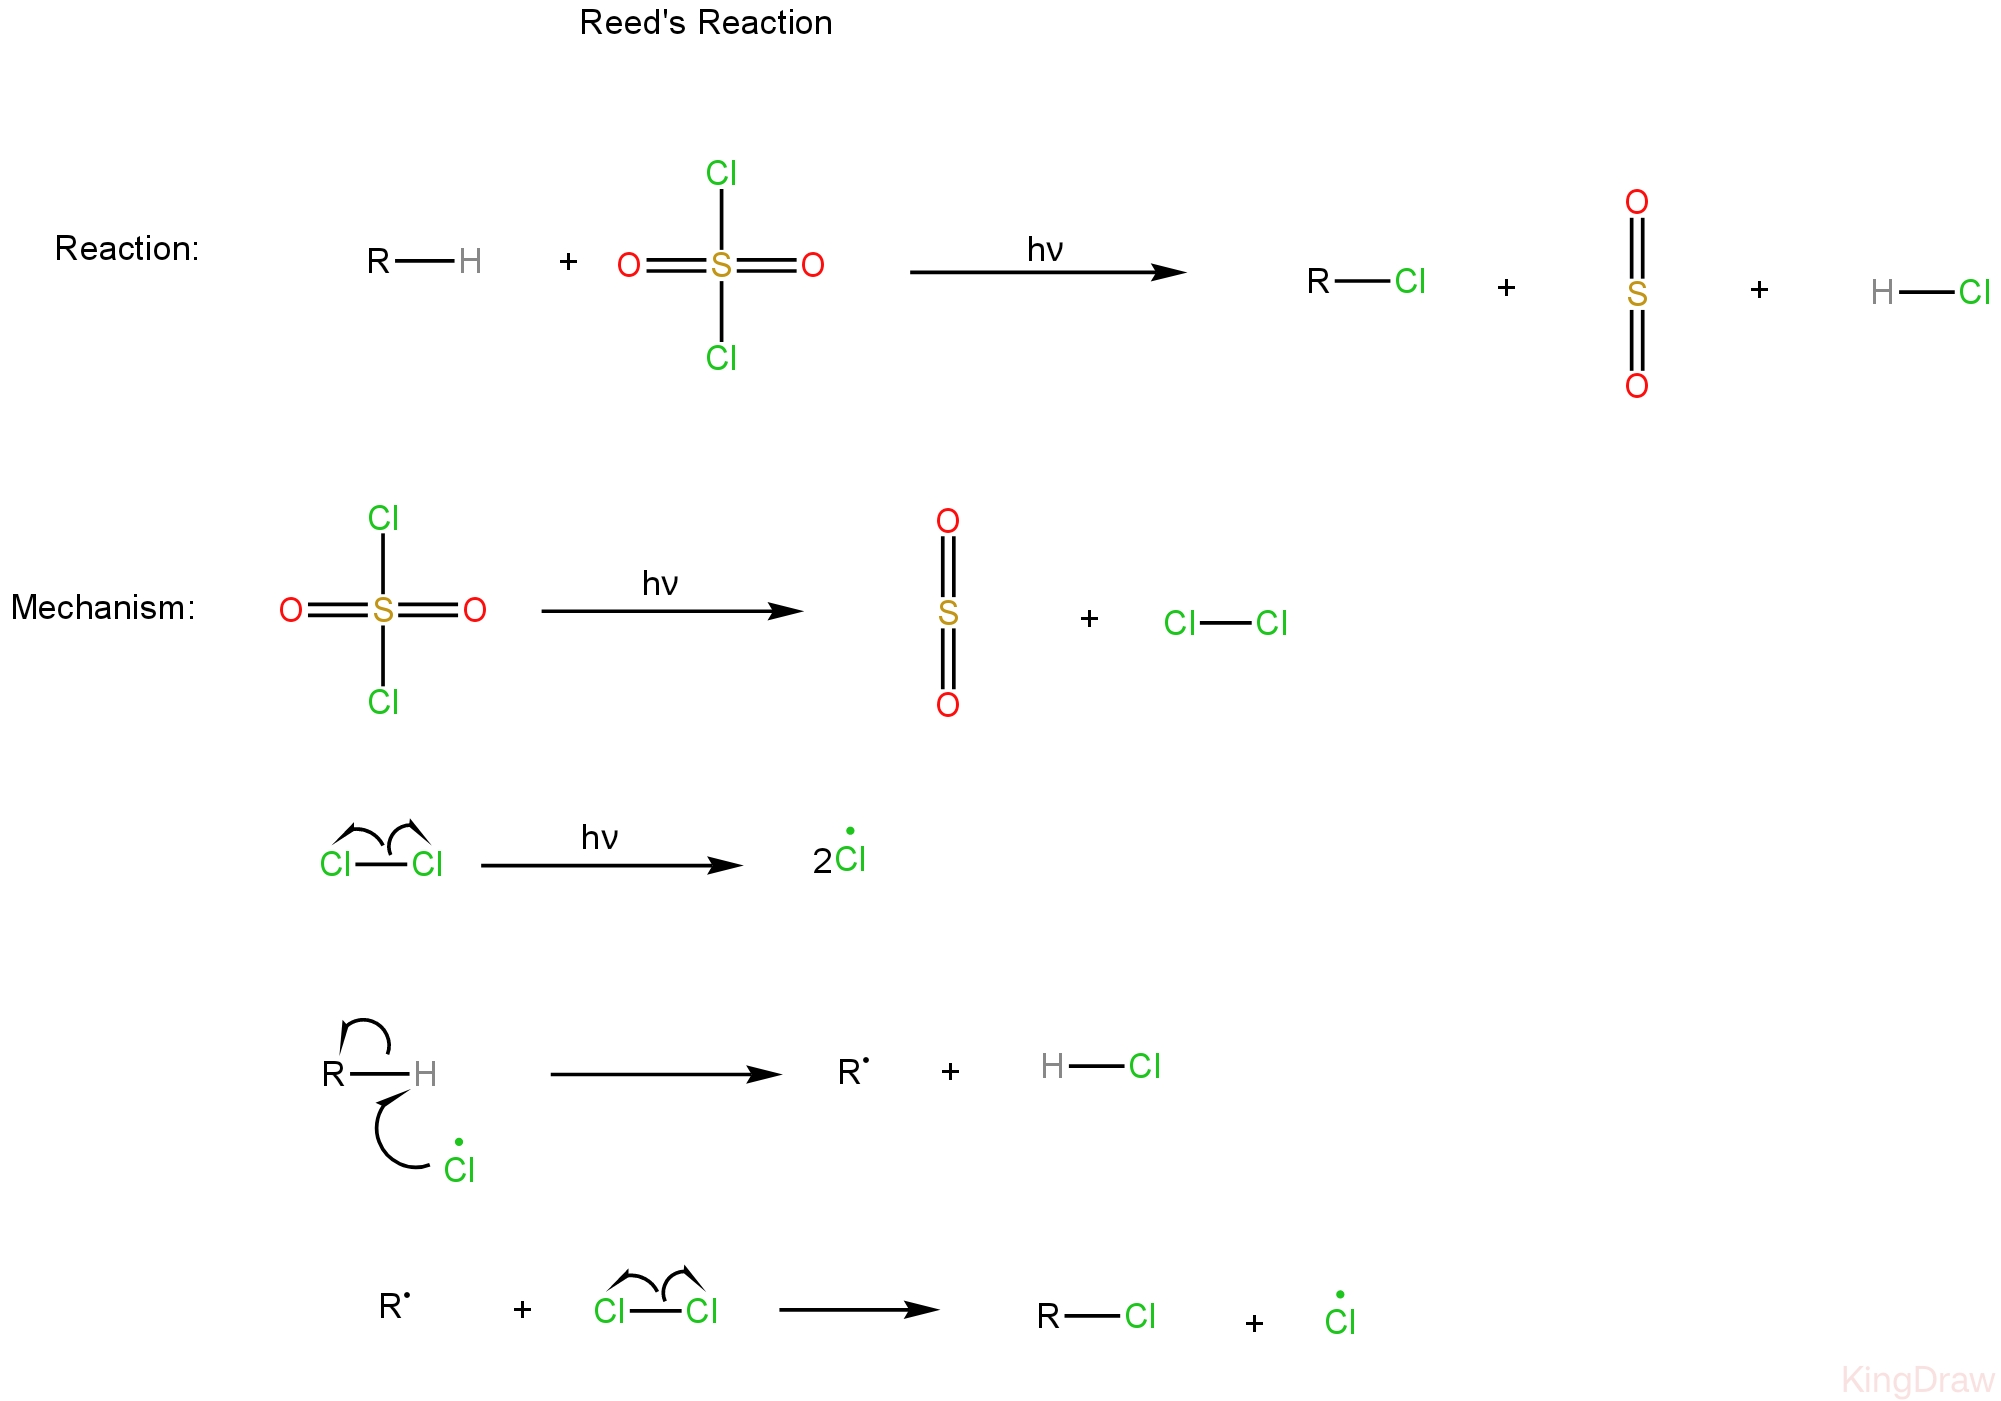
\includegraphics[scale=0.22]{Reed'sReaction_1722185097608.JPEG}
\end{center}

\section{NBS}
\subsection{Reaction and Mechanism}
\begin{center}
    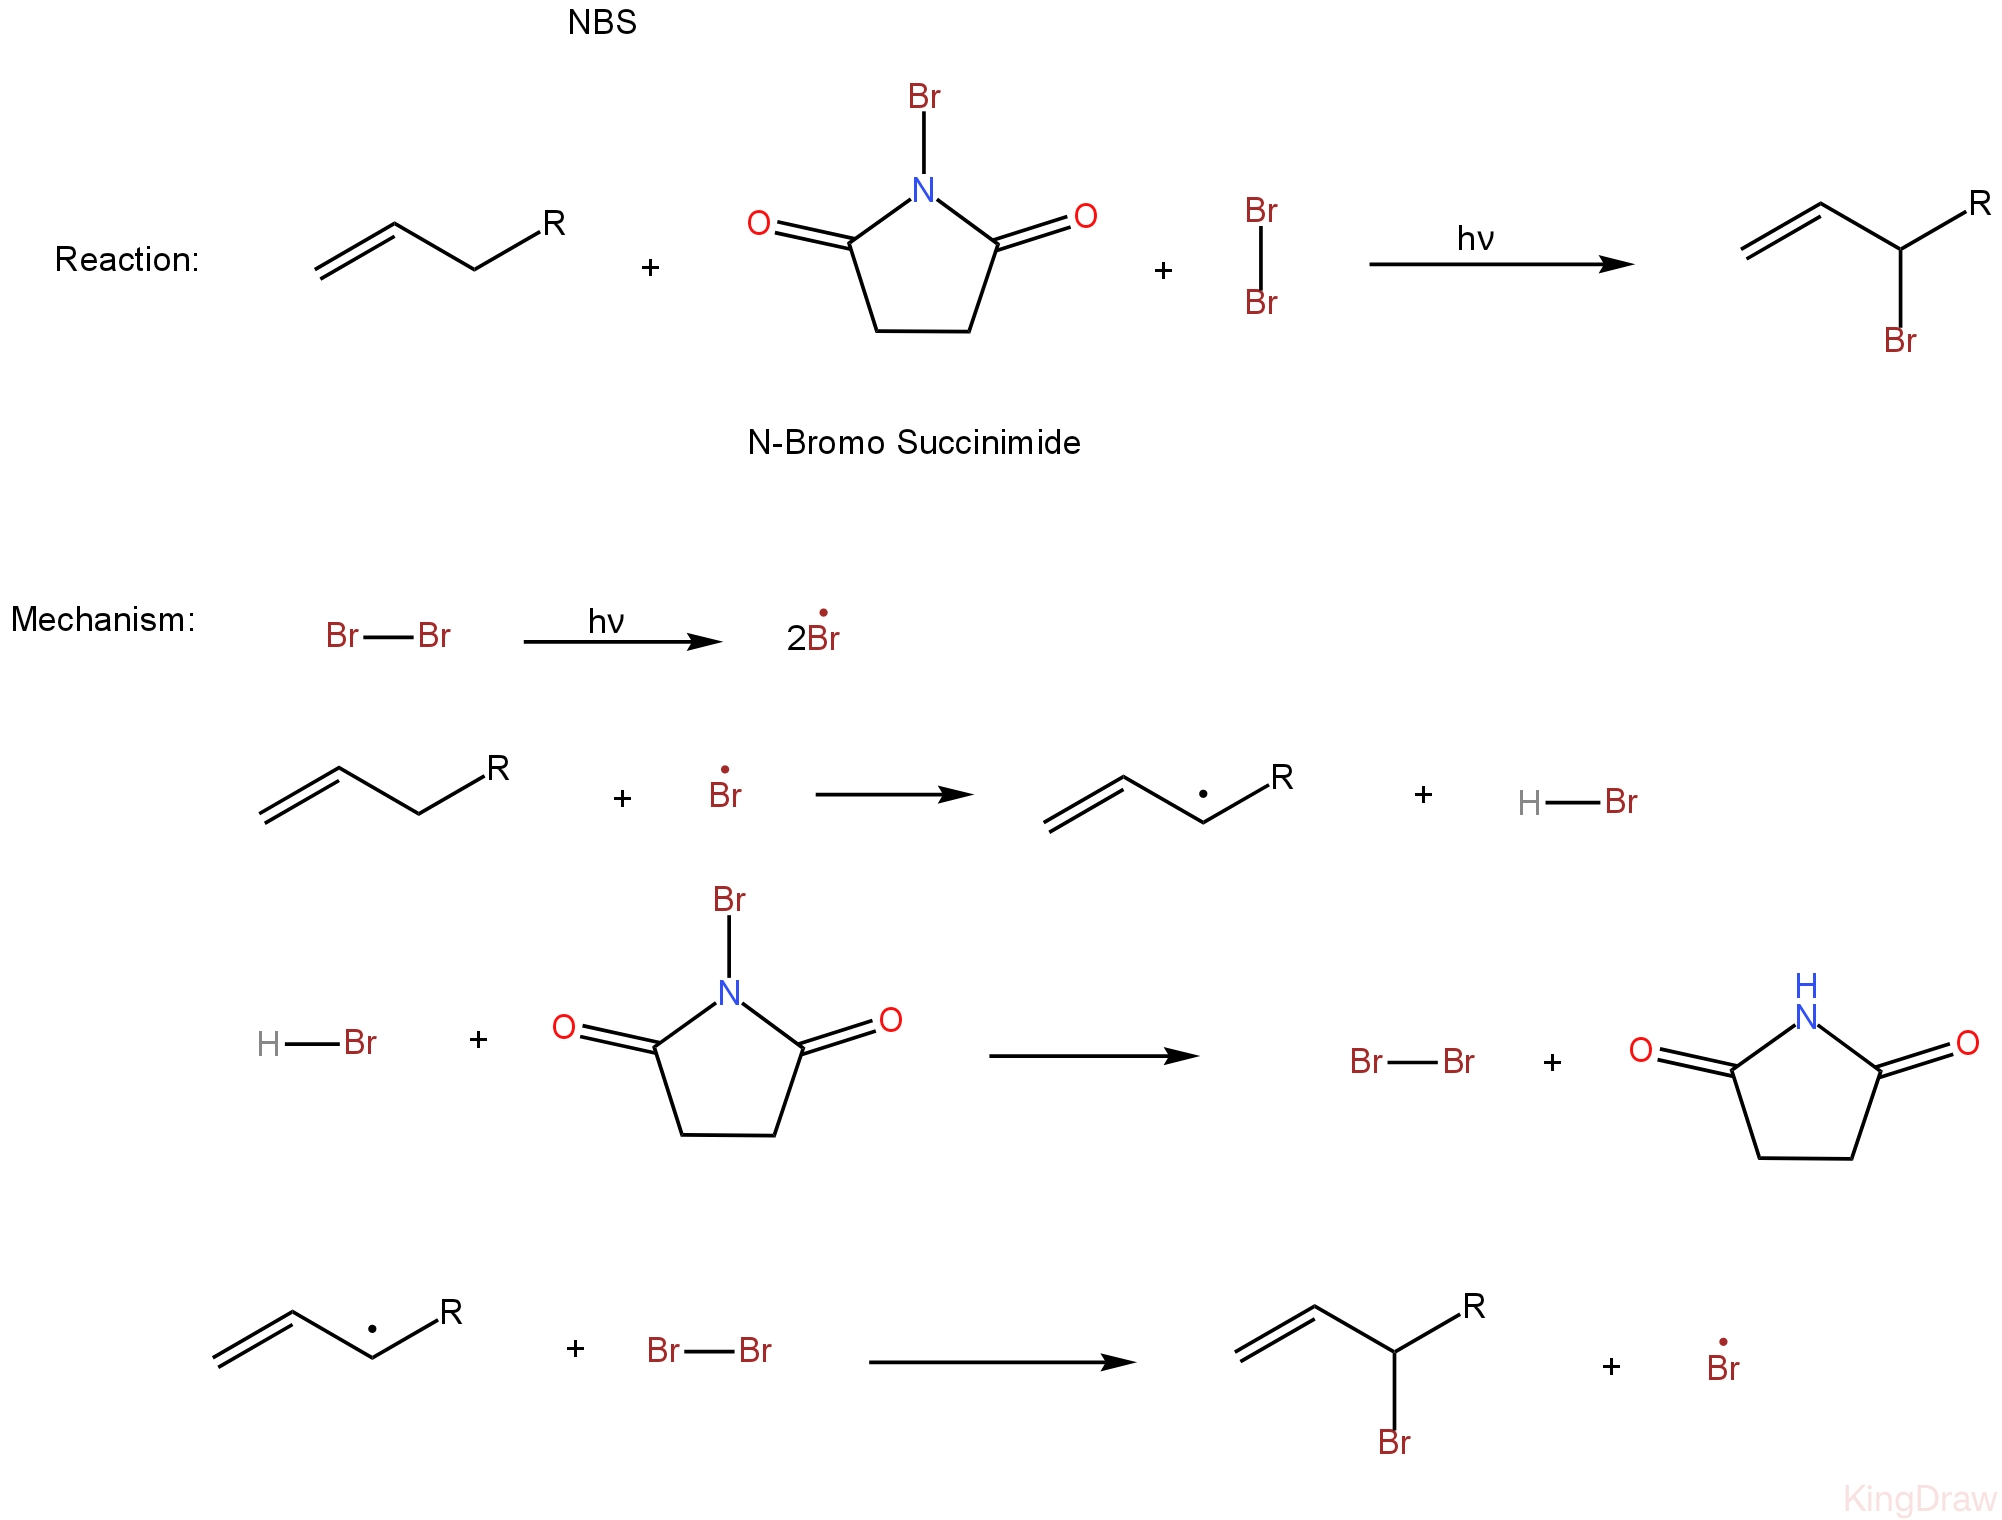
\includegraphics[scale=0.22]{NBS.JPEG}
\end{center}
\subsection{Reaction Observations}
\begin{enumerate}[i.]
    \item Reacts only with Allylic and Benzylic positions.
    \item $C^{\fullcirc}$ obtained as intermediate.
    \item Example of Substitution Reaction.
    \item Pure NBS is inert, hence, impurity of $HBr$ or $Br_{2}$ is added.
    \item Example of Oxidation Reaction.
\end{enumerate}

\section{Electrophilic Addition Reaction}
\subsection{Reaction and Mechanism}
\begin{center}
    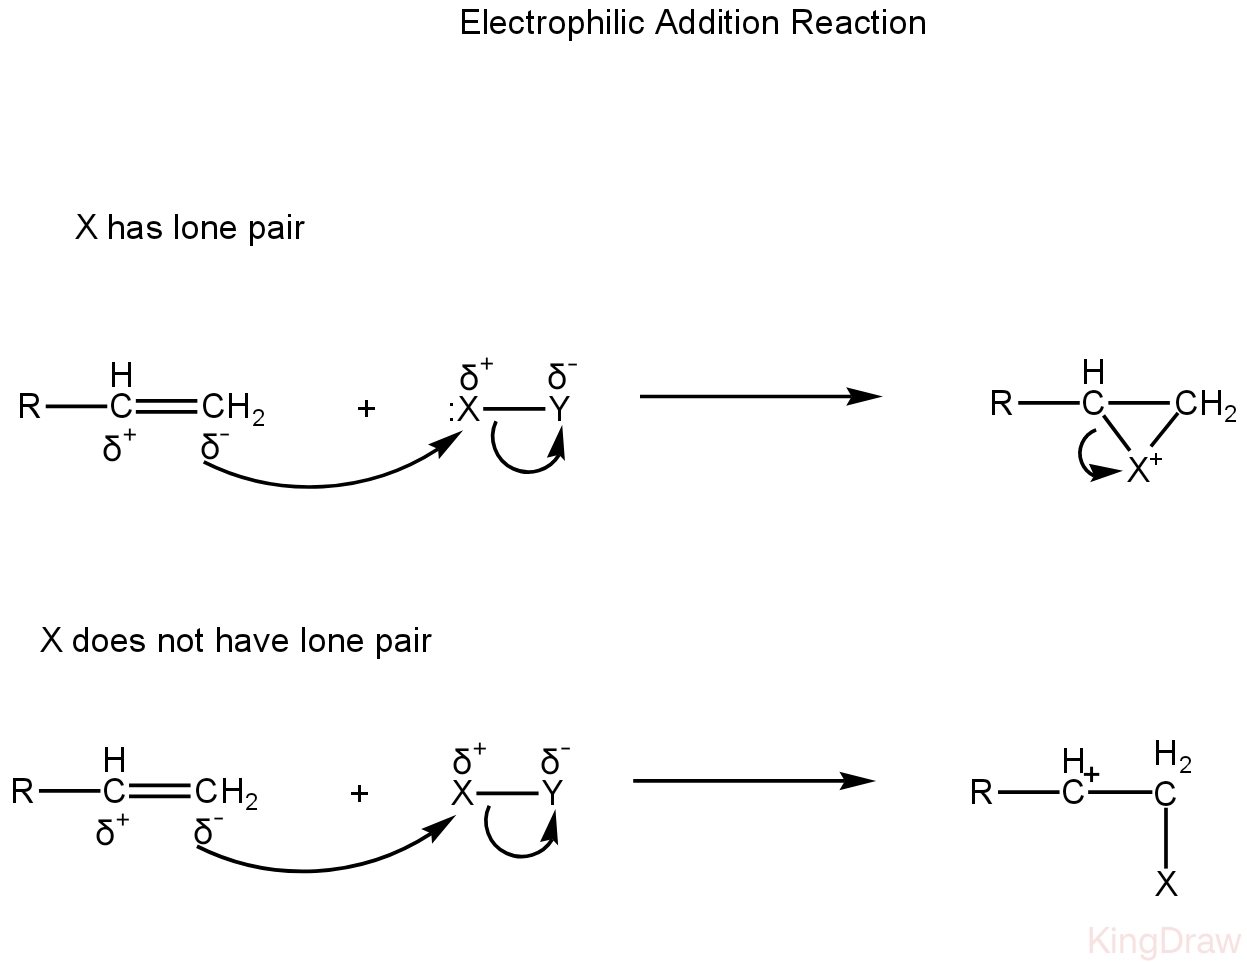
\includegraphics[scale=0.3]{ElectrophilicAdditionReaction_1722210371705.JPEG}
\end{center}
\subsection{Reaction Observations}
\subsection{$X$ doesn't have lone pair}
\begin{enumerate}[i.]
    \item $C^+$ obtained as intermediate.
    \item Rearrangement can occur.
\end{enumerate}
\subsection{$X$ has lone pair}
\begin{enumerate}[i.]
    \item Non Classical Carbocation (NCC or Cyclohalonium ion) obtained as intermediate.
    \item No Rearrangement.
\end{enumerate}
\subsection{Reagent Table}

\begin{tabular}{|c| c| c| c| }
    \hline
    Reagent                                         & $E^+$  & $Nu^-$             & Path                   \\[1mm]
    \hline
    $HCl, HBr, HI$                                  & $H^+$  & $Cl^-, Br^-, I^-$  & $X$ does not lone pair \\
    $DCl$                                           & $D^+$  & $Cl^-$             & $X$ does not lone pair \\
    $H^+/H_{2}O, H_{3}O^+, \text{dil.} H_{2}SO_{4}$ & $H^+$  & $OH^-$             & $X$ does not lone pair \\
    $ROH/H^+$                                       & $H^+$  & $OR^-$             & $X$ does not lone pair \\
    $RCOOH/H^+$                                     & $H^+$  & $RCOO^-$           & $X$ does not lone pair \\
    \hline
    $X_{2}/CCl_{4}$                                 & $X^+$  & $X^-$              & $X$ has lone pair      \\
    $Br_{2}/H_{2}O$ or $HOBr$                       & $Br^+$ & $Br^-, OH^-$       & $X$ has lone pair      \\
    $Br_{2}/H_{2}O$ in Brine                        & $Br^+$ & $Br^-, OH^-, Cl^-$ & $X$ has lone pair      \\
    $NOCl$ (Tilden Reagent)                         & $NO^+$ & $Cl^-$             & $X$ has lone pair      \\
    $IN_{3}$                                        & $I^+$  & $N_{3}^-$          & $X$ has lone pair      \\
    \hline
\end{tabular}

\subsection{KCP and TCP}
\begin{center}
    \begin{tabular}{c | c}
        KCP                                                 & TCP                                  \\
        Kinetically Controlled Product                      & Thermodynamically Controlled Product \\
        $1,2-$ Product is assumed to be KCP                 & Can be $1,2 $ and $1,4$              \\
        Fast Rate                                           & Stable Product                       \\
        Favors at low temperature ($-80, -40, 0 ^ \circ C$) & Favors high temperature
    \end{tabular}
\end{center}

\section{Oxymercuration Demercuration}
\subsection{Reaction and Mechanism}
\begin{center}
    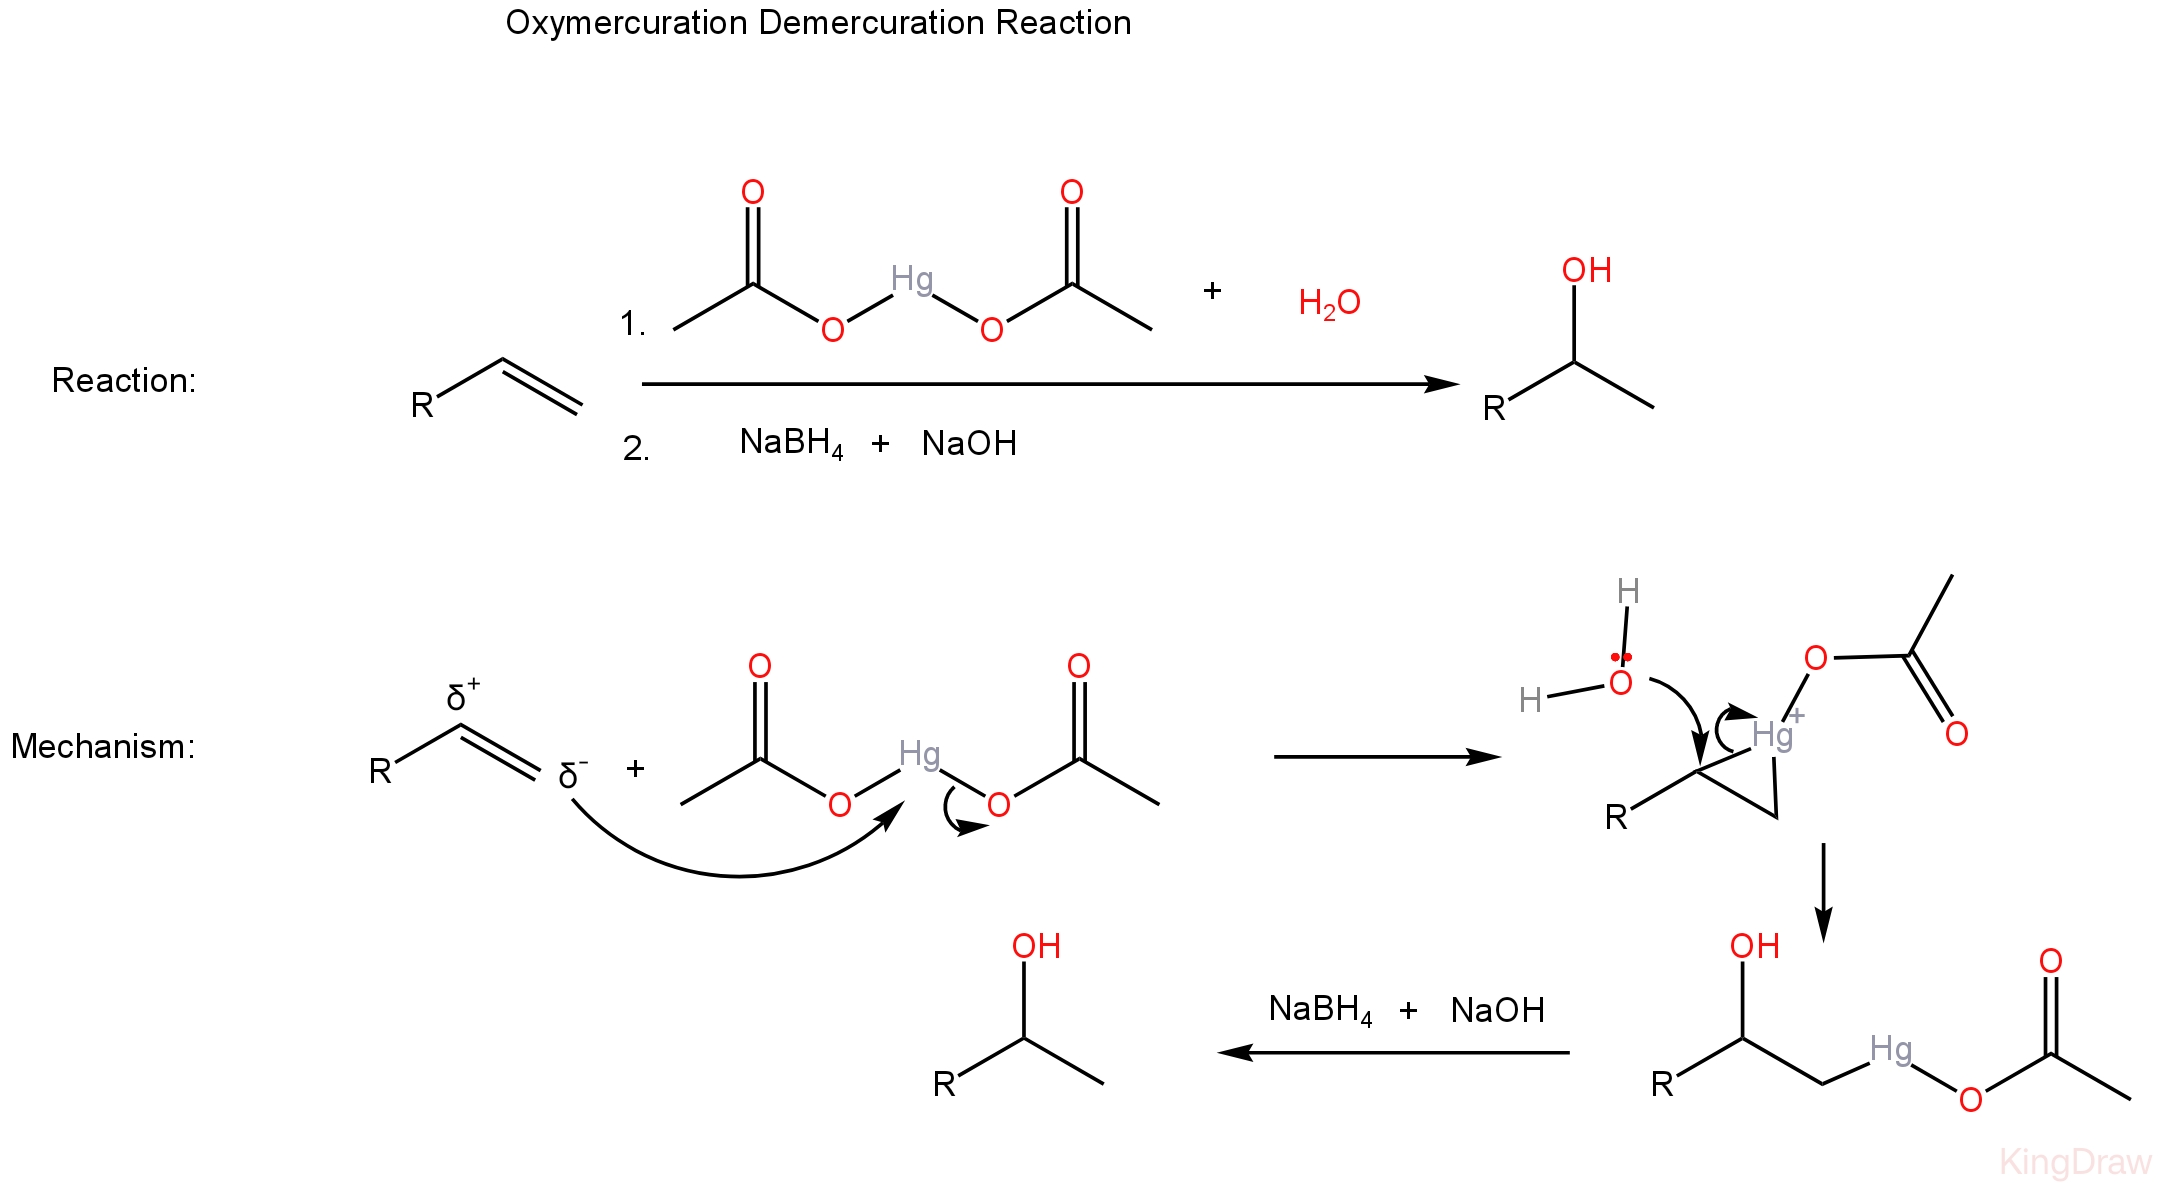
\includegraphics[scale=0.22]{OMDM_1722369977375.JPEG}
\end{center}
\subsection{Reaction Observations}
\begin{enumerate}[i.]
    \item Markonikov addition.
    \item No rearrangment.
    \item Both Syn and anti addition.
    \item OM is anti additon, DM involves $C^{\fullcirc}$, hence both syn and anti addition.
    \item Metal $Hg^{\fullcirc}$ is obtained.
\end{enumerate}

\section{Iodolactonization}
\subsection{Reaction and Mechanism}
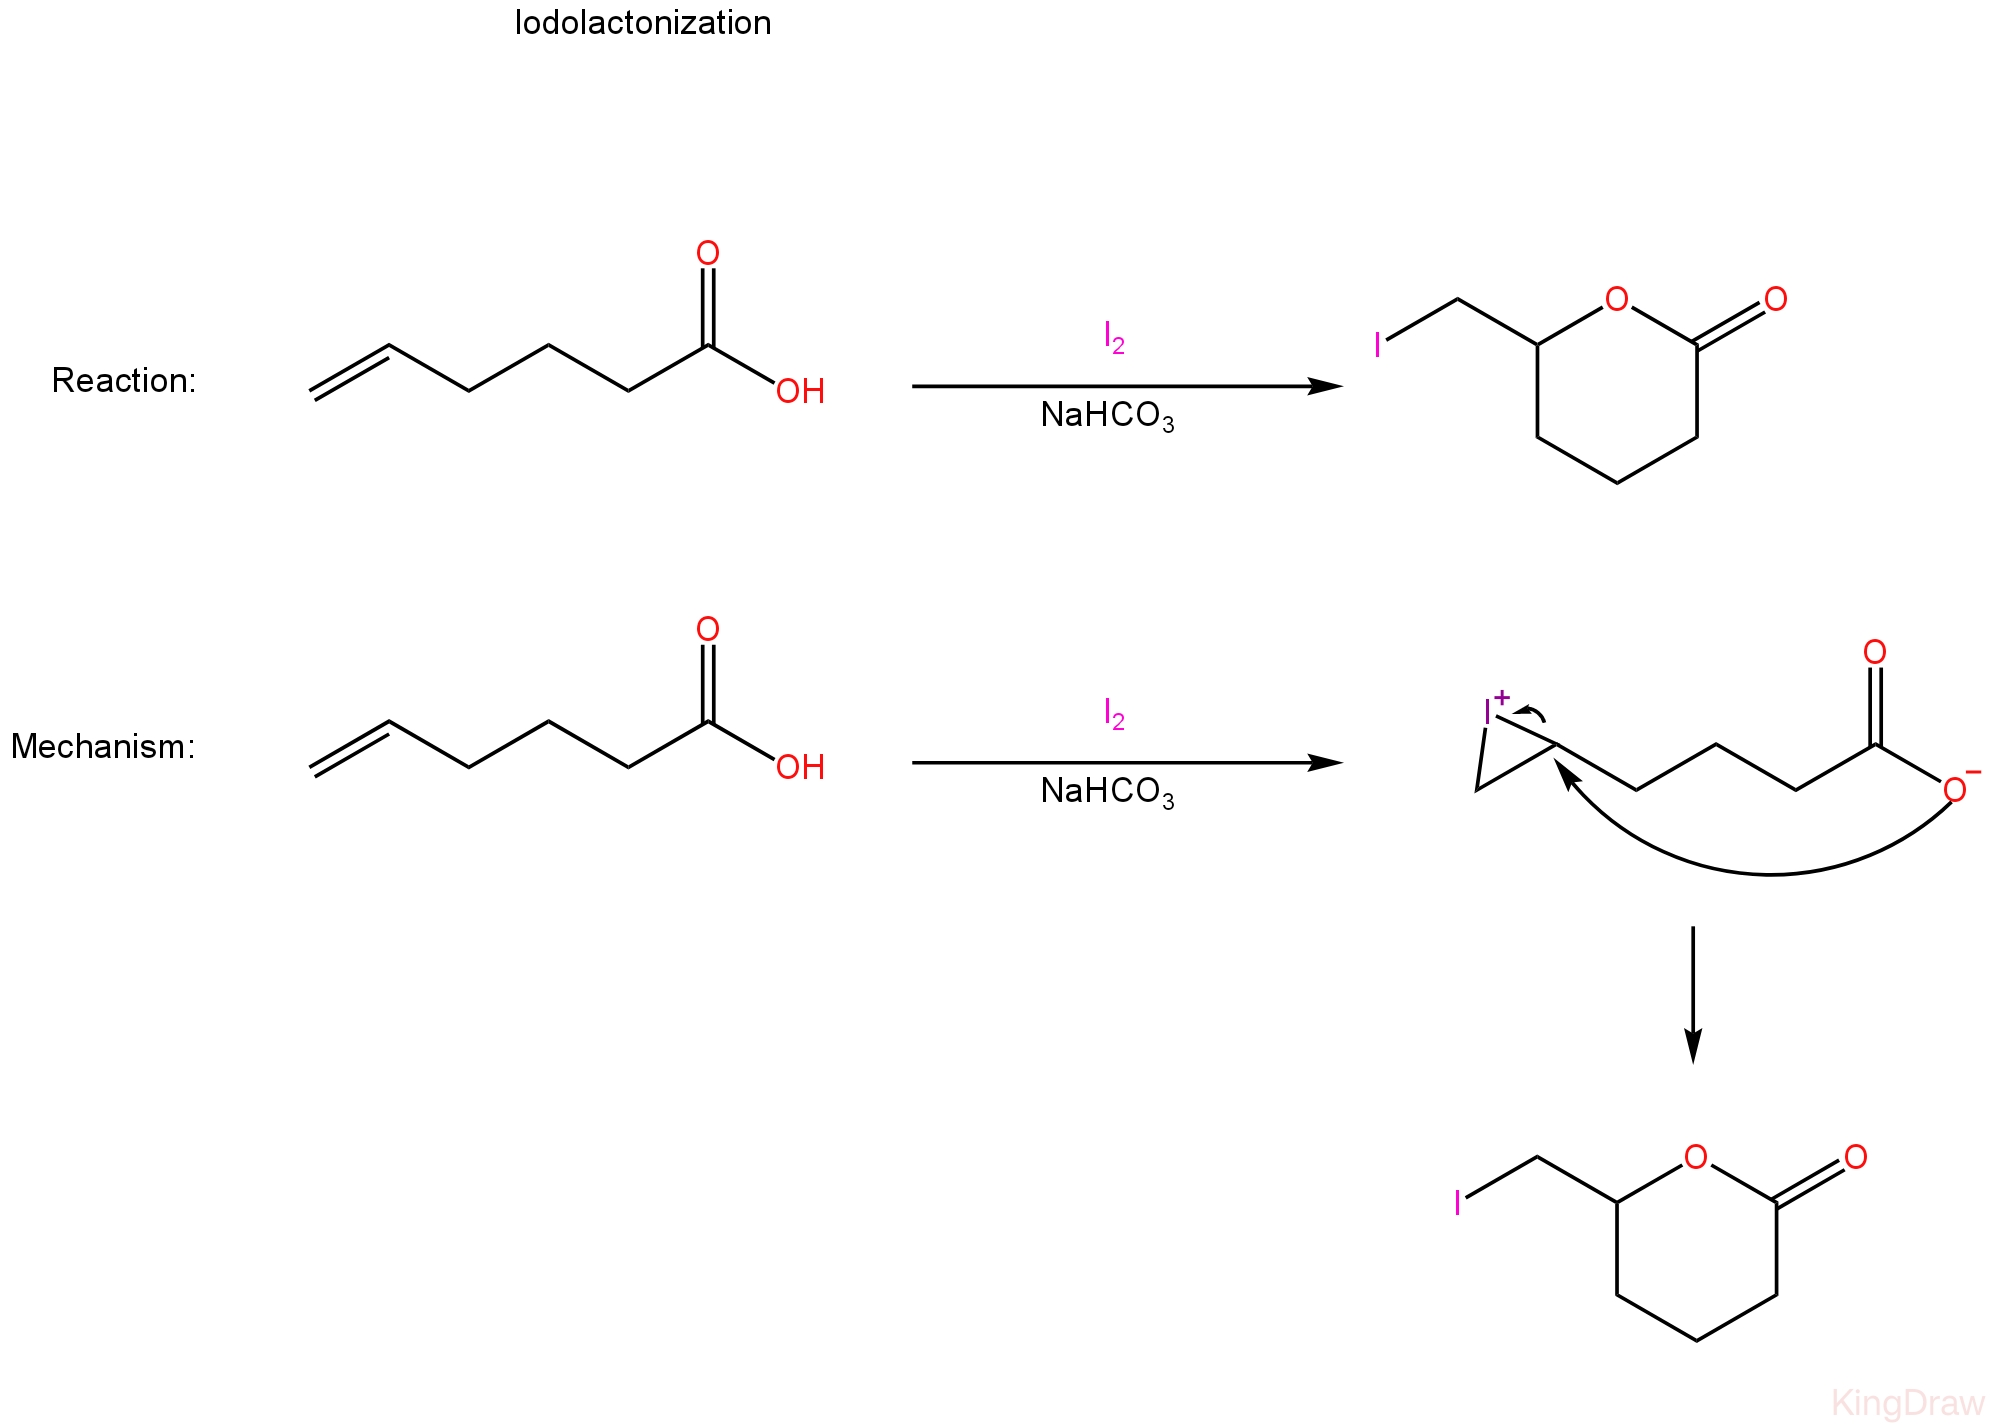
\includegraphics[scale=0.23]{Iodolactonization_1722375521493.JPEG}

\section{Kuchrov's Reaction}
\subsection{Reaction and Mechanism}
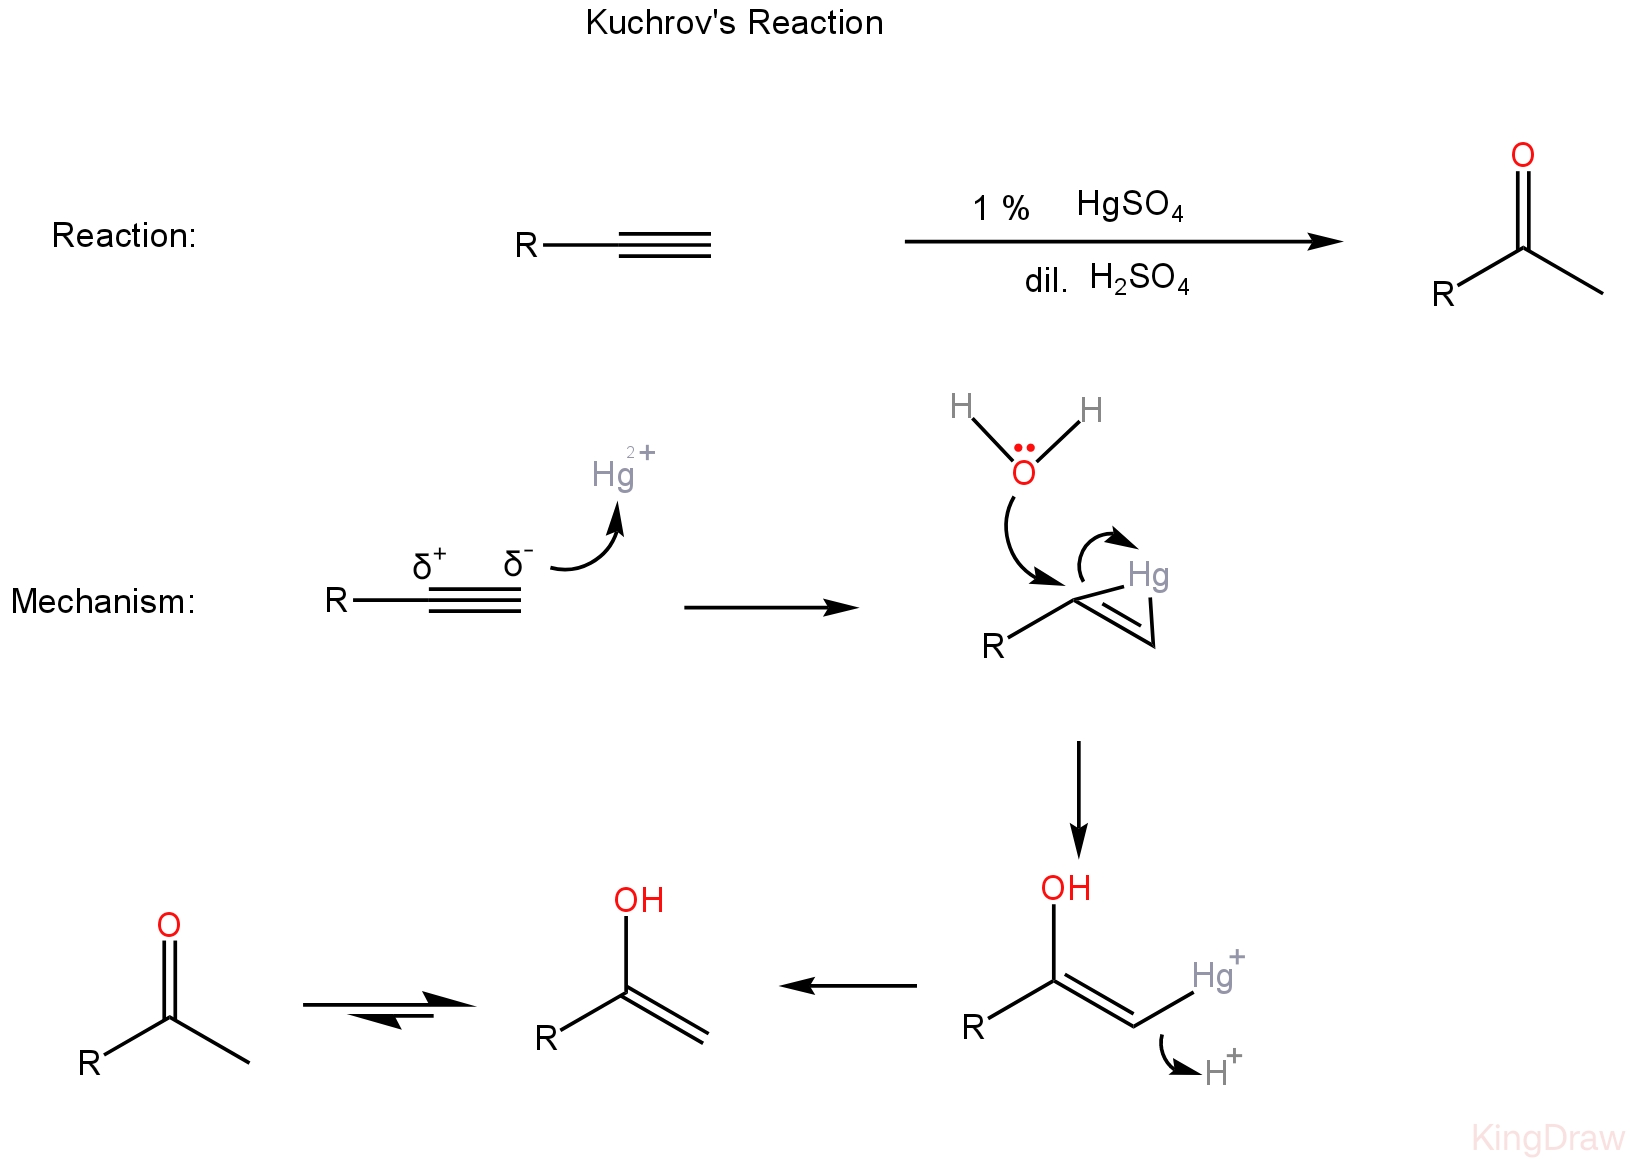
\includegraphics[scale=0.26]{Kuchrov_1722377904329.JPEG}
\subsection{Reaction Observations}
\begin{enumerate}[i.]
    \item Example of Electrophilic Additon Reaction.
    \item NCC type intermediate is obtaied.
    \item Involves tautomerism.
    \item Mixed carbony are obtaied.
\end{enumerate}

\section{Kharasch Effect}
\subsection{Reaction and Mechanism}
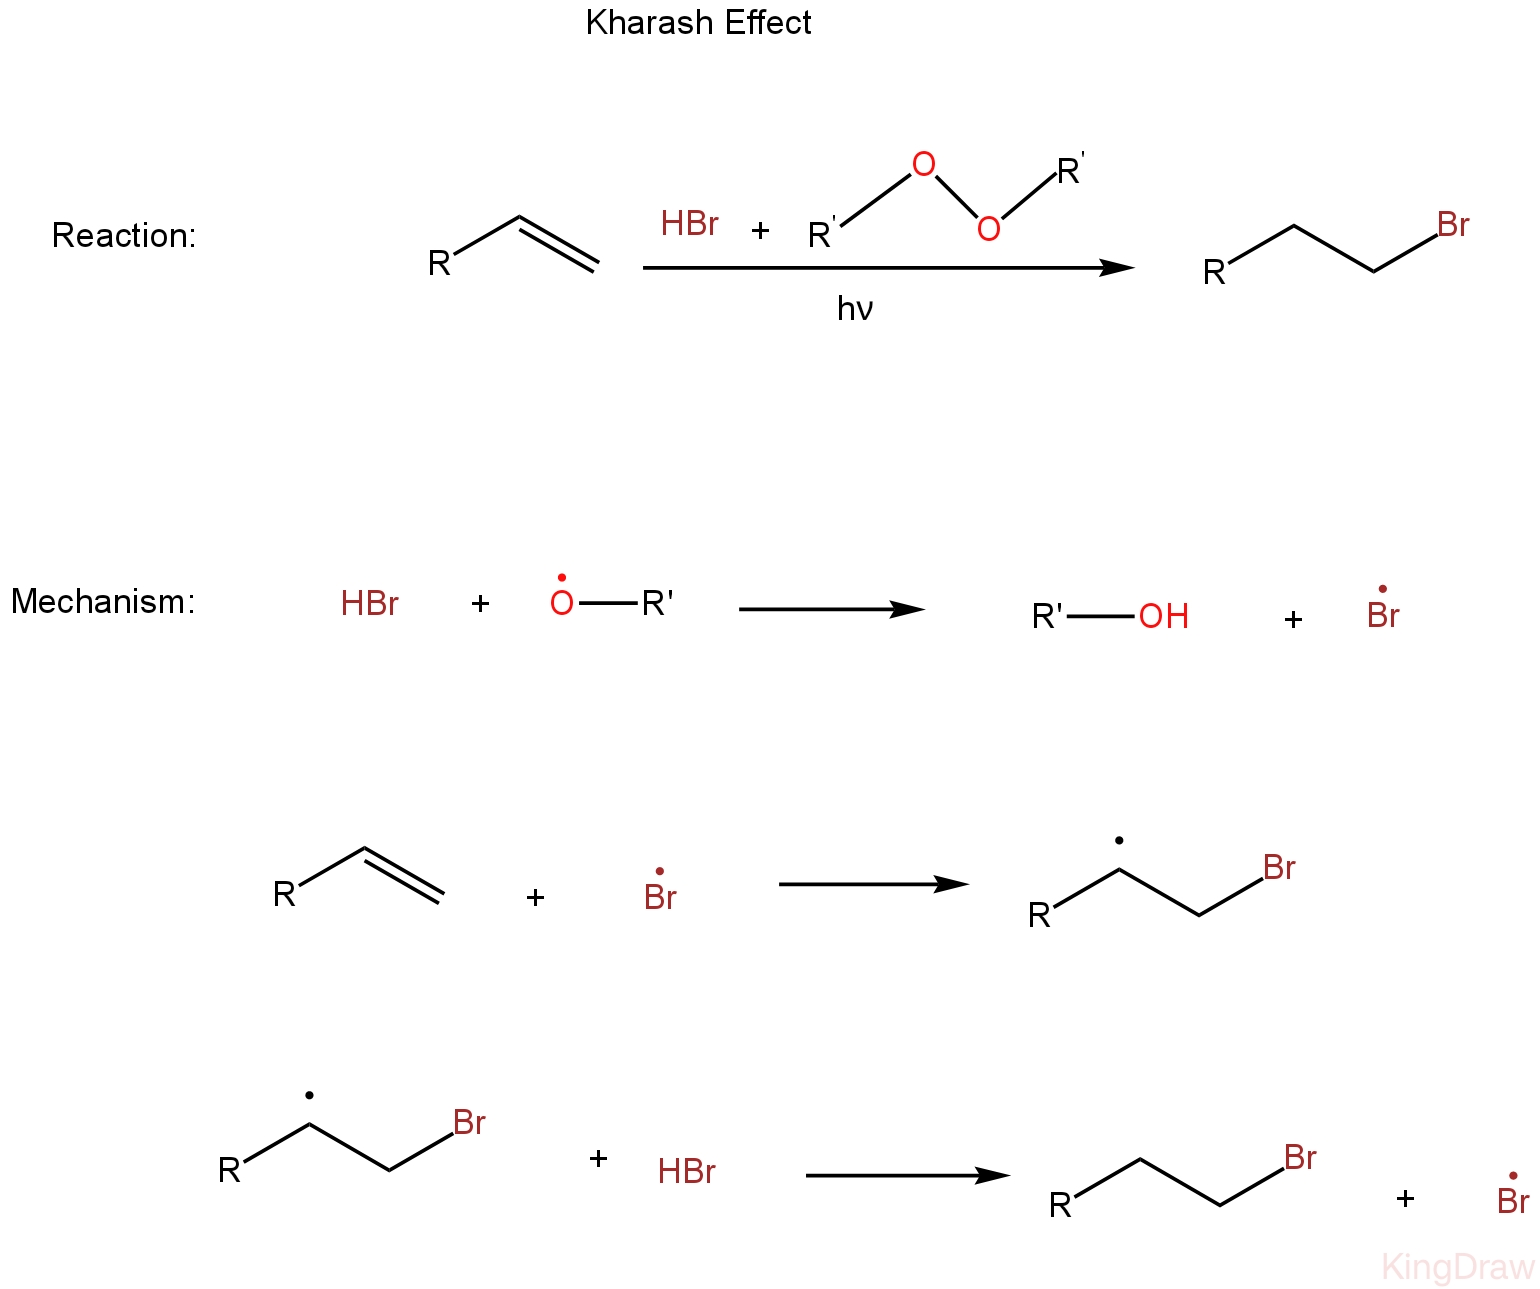
\includegraphics[scale=0.27]{KharaschEffect_1722410819316.JPEG}
\subsection{Reaction Observations}
\begin{enumerate}[i.]
    \item $C^{\fullcirc}$ obtained as intermediate.
    \item Example of $C^{\fullcirc}$ addition Reaction.
    \item Anti-markonikov addition
    \item Only $HBr$ shows peroxide effect (Kharasch Effect).
\end{enumerate}

\section{Catalytic Hydrogenation}
\subsection{Reaction and Mechanism}
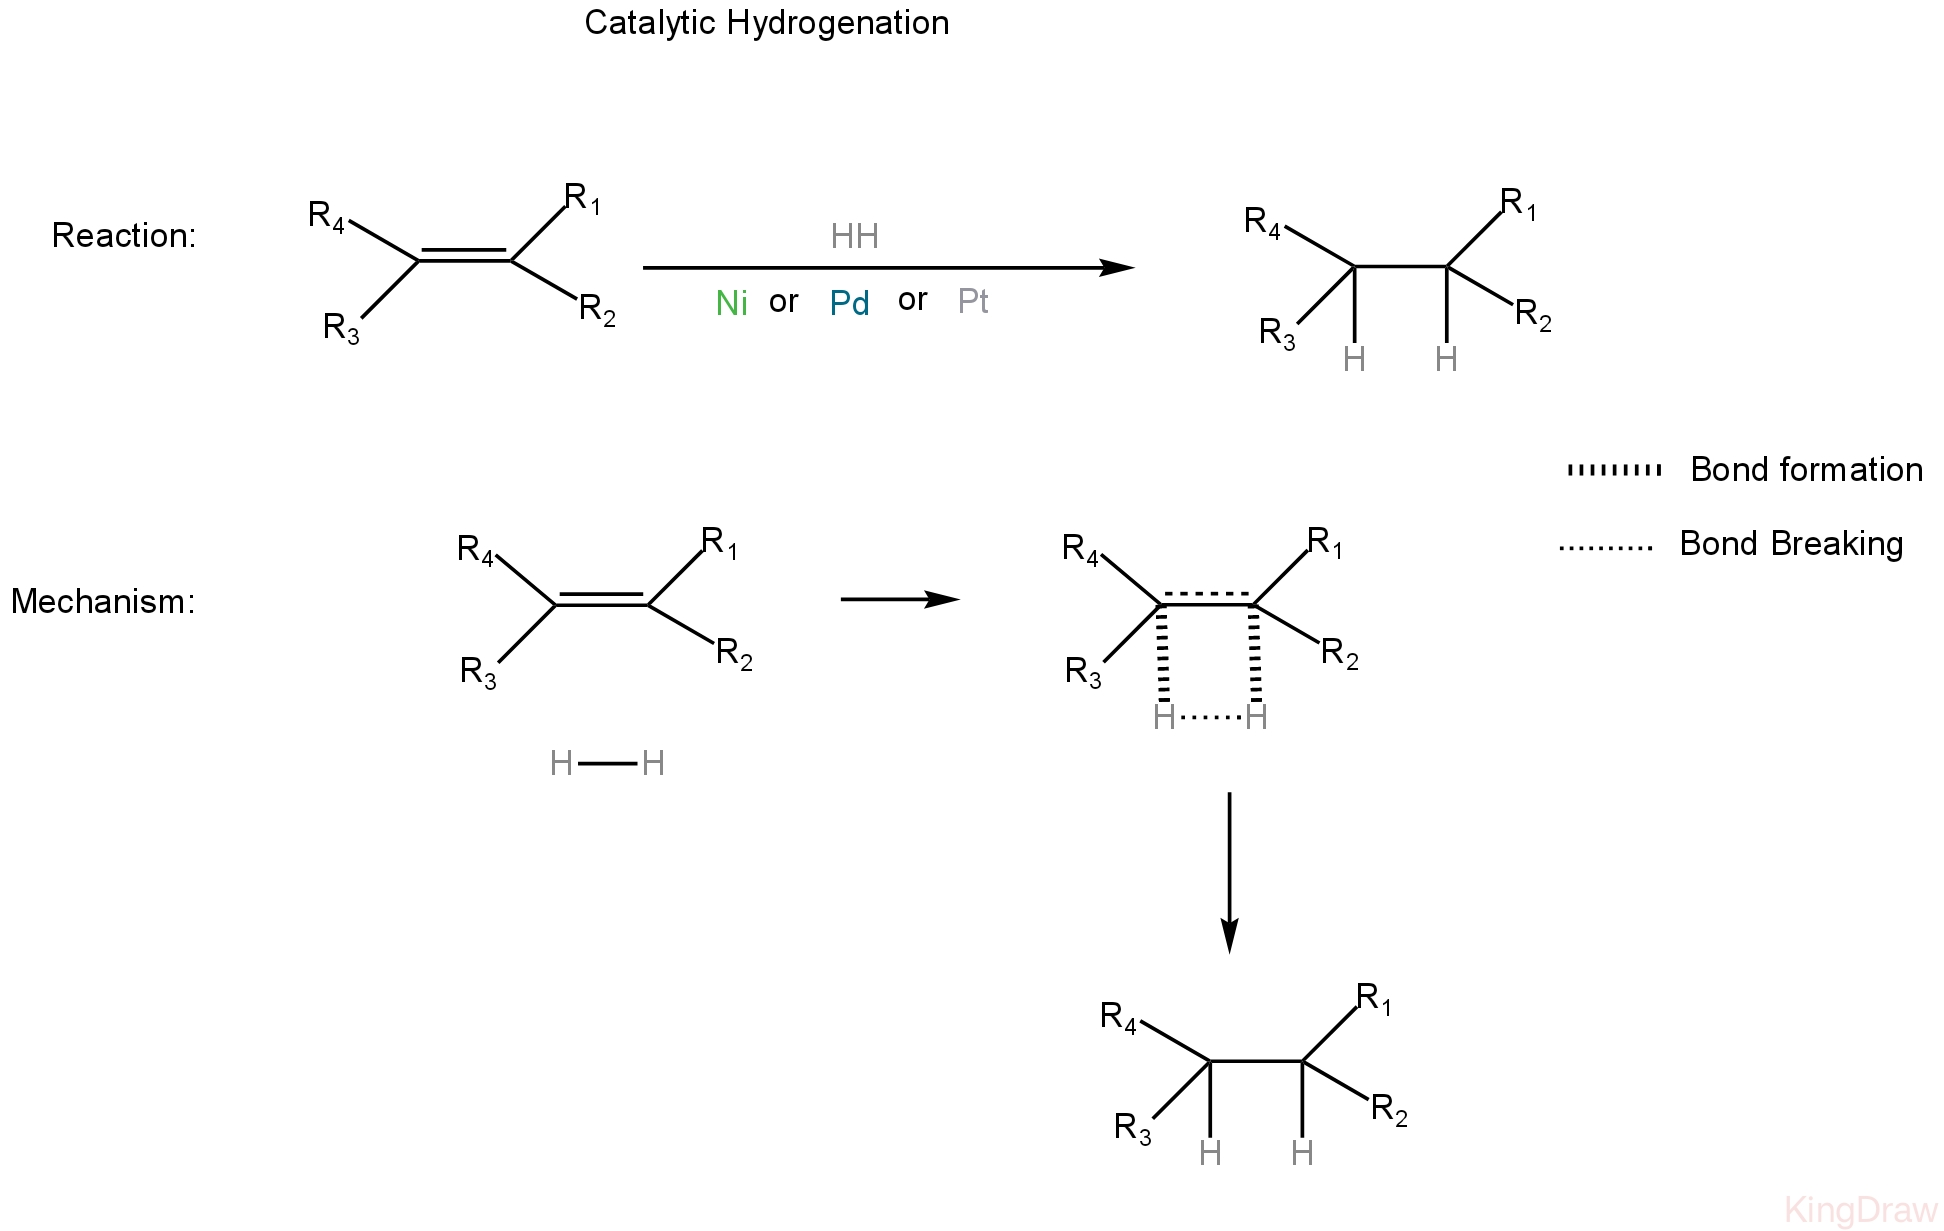
\includegraphics[scale=0.24]{p_jpg.JPEG}
\subsection{Reaction Observations}
\begin{enumerate}[i.]
    \item Example of additon and Redox reaction.
    \item syn additon
    \item Example of surface phenomenon and involvs $4$ MCTS.
    \item $Pd / BaSO_{4}$ a.k.a Lindlar's Catalyst and Quinoline is added as poison.
    \item In case of conjugated diene, 1,4addition takes place due to $6$ MCTS.
    \item Reactivity, \\
          $C-S$ bond $>$ Alkyne $> Ar-NO_{2} > R-COCl>$ Alkene $> RCHO> RCOR> \textit{Benzene}^*>RCOOH^*< \textit{acid derivative}^* \hfill * \text{require heat}$

          $\propto \dfrac{1}{\text{Steric Hindrance}}$

          $\propto \dfrac{1}{\text{Stability of Alkene}}$
\end{enumerate}

\section{Rosenmund Reaction}
$$on hold$$

\section{Hydroboration Oxidation}
\subsection{Reaction and Mechanism}
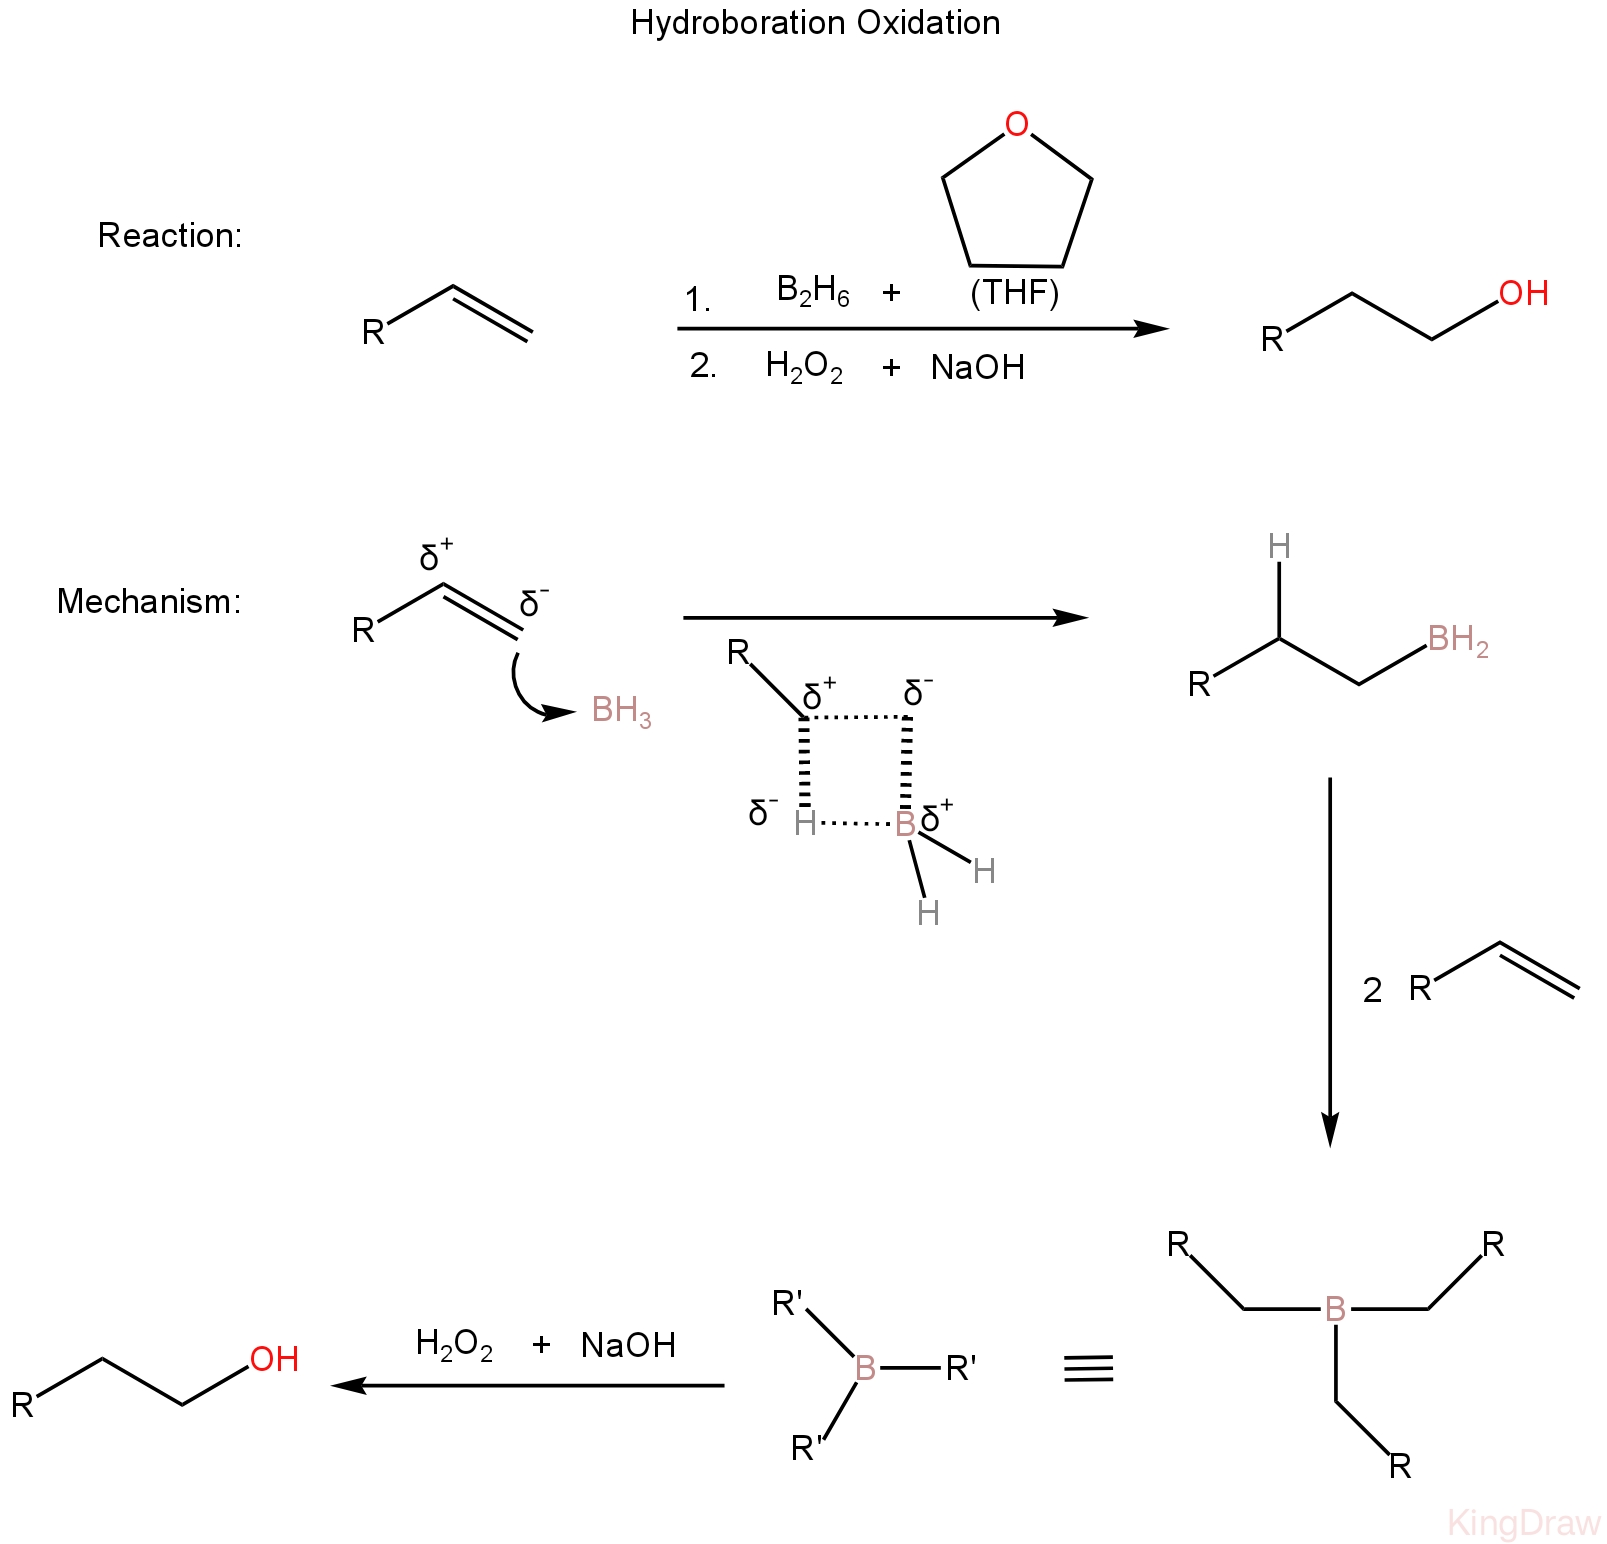
\includegraphics[scale=0.25]{hbo_1722684553916.JPEG}
\subsection{Reagent Table}
\begin{tabular}{|c|c | c|}
    \hline
    Reactant  & Reagent           & Product  \\
    \hline
    $R'_{3}B$ & $H_{2}O_{2}/NaOH$ & $3 R'OH$ \\
              & $H_{2}O$          & $3R'H$   \\
              & $RCOOH$           & $3R'H$   \\
              & $Cl_{2}$          & $3R'Cl$  \\
    \hline
\end{tabular}
\subsection{Reaction Observations}
\begin{enumerate}[i.]
    \item Sys addition.
    \item Anti-markonikov addition.
    \item Involvs 4MCTS.
    \item In case of acid or water, reduction occurs.
    \item Generally, $3 \hspace{2mm} mol.$ alkene is required for $1 \hspace{2mm} mol. \hspace{2mm} BH_{3} $
    \item $9-BBN, \hspace{2mm}Sia_{2}BH$ is used for selective addition on less crowded terminal alkene.
\end{enumerate}

\section{Birch Reduction}
\subsection{Reaction and Mechanism}
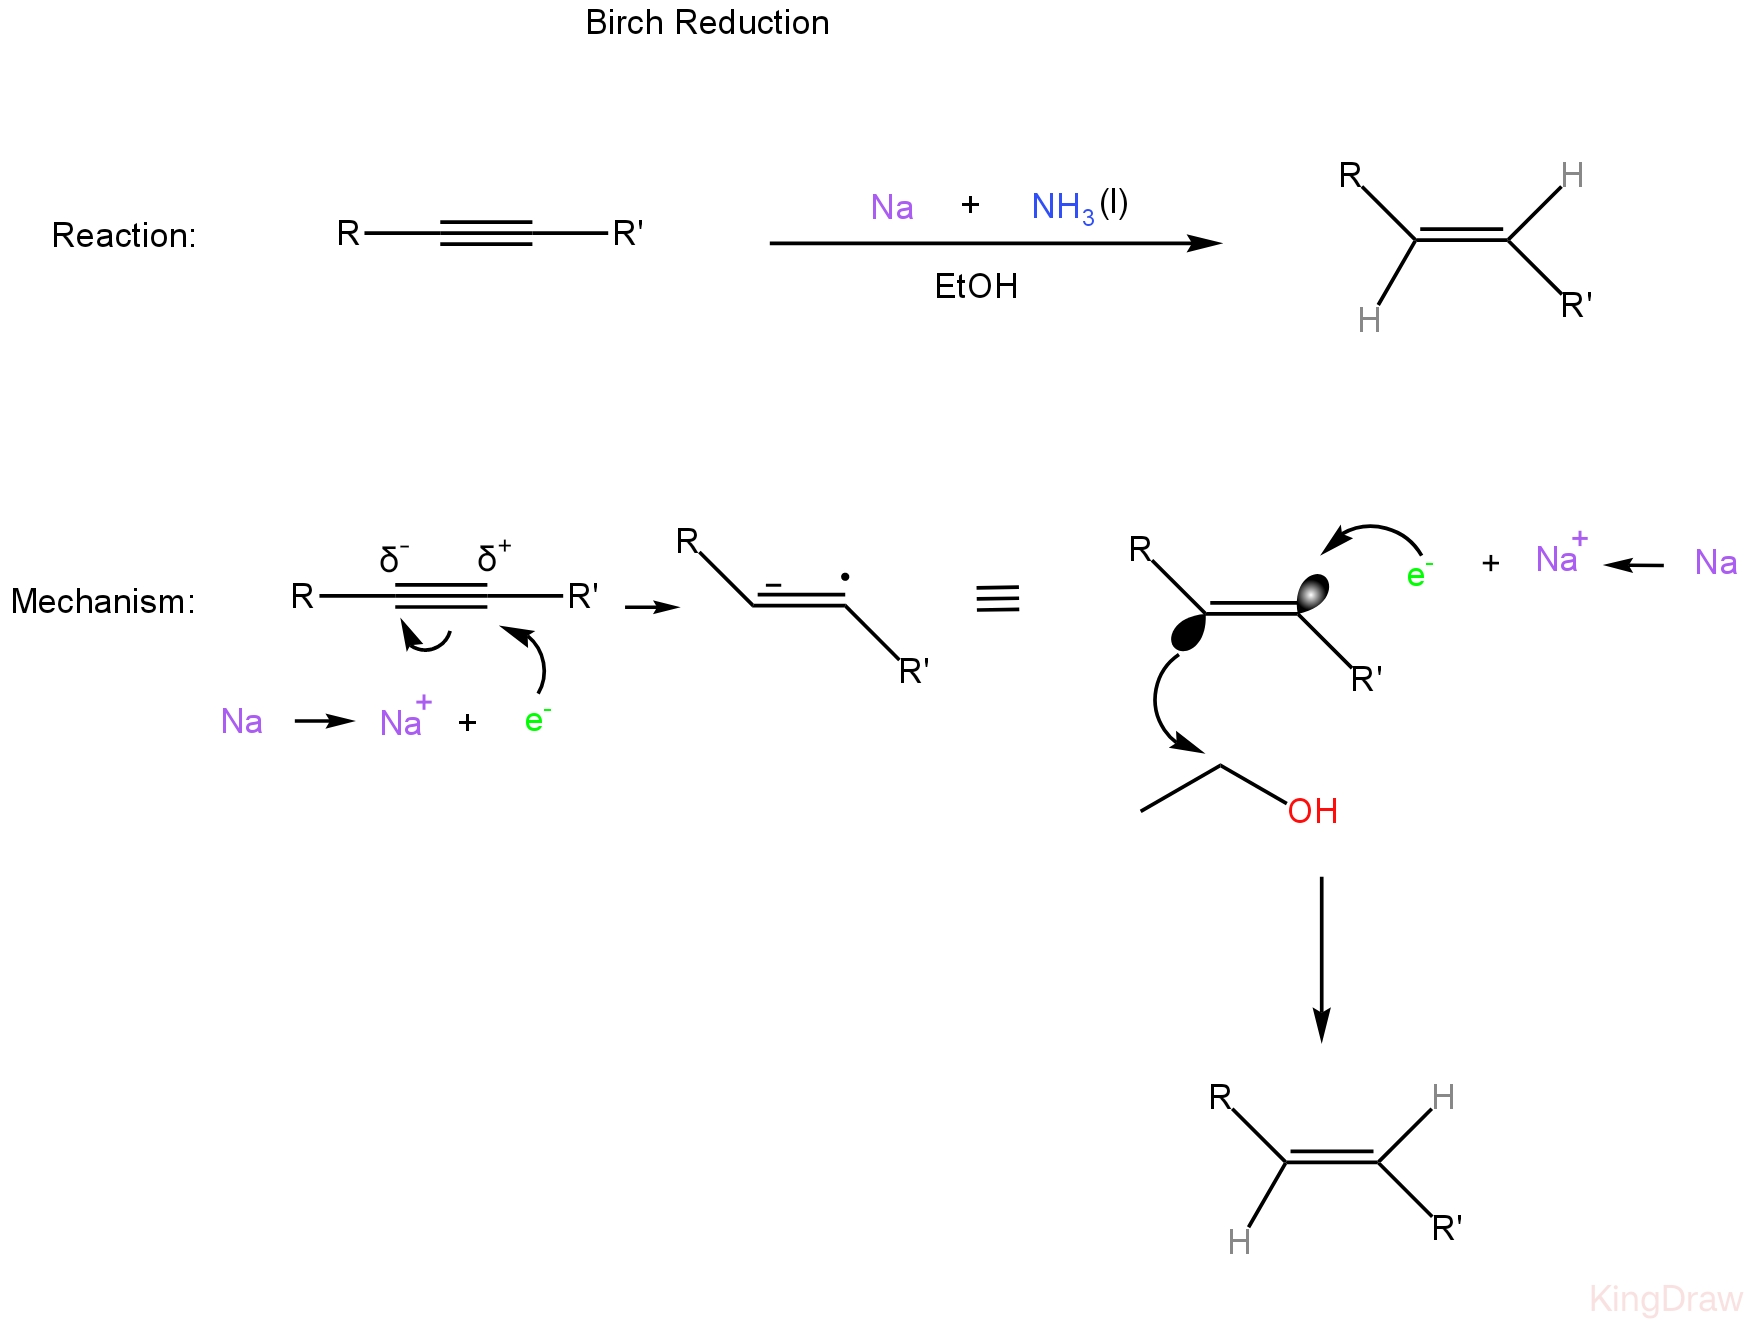
\includegraphics[scale=0.25]{birch_1722686860261.JPEG}
\subsection{Reaction Observations}
\begin{enumerate}[i.]
    \item $Na/ NH_{3}(l)$ is a blue color solution.
    \item Both $C^{\fullcirc}$ and $C^-$ obtained as intermediate.
    \item $ROH$ is used as proton source.
    \item Terminal Alkyne will not give alkene, acid base reaction will occur.
    \item In case of substituted benzene, more stable alkene is major product.
\end{enumerate}
\section{Oxidation of Alkene}

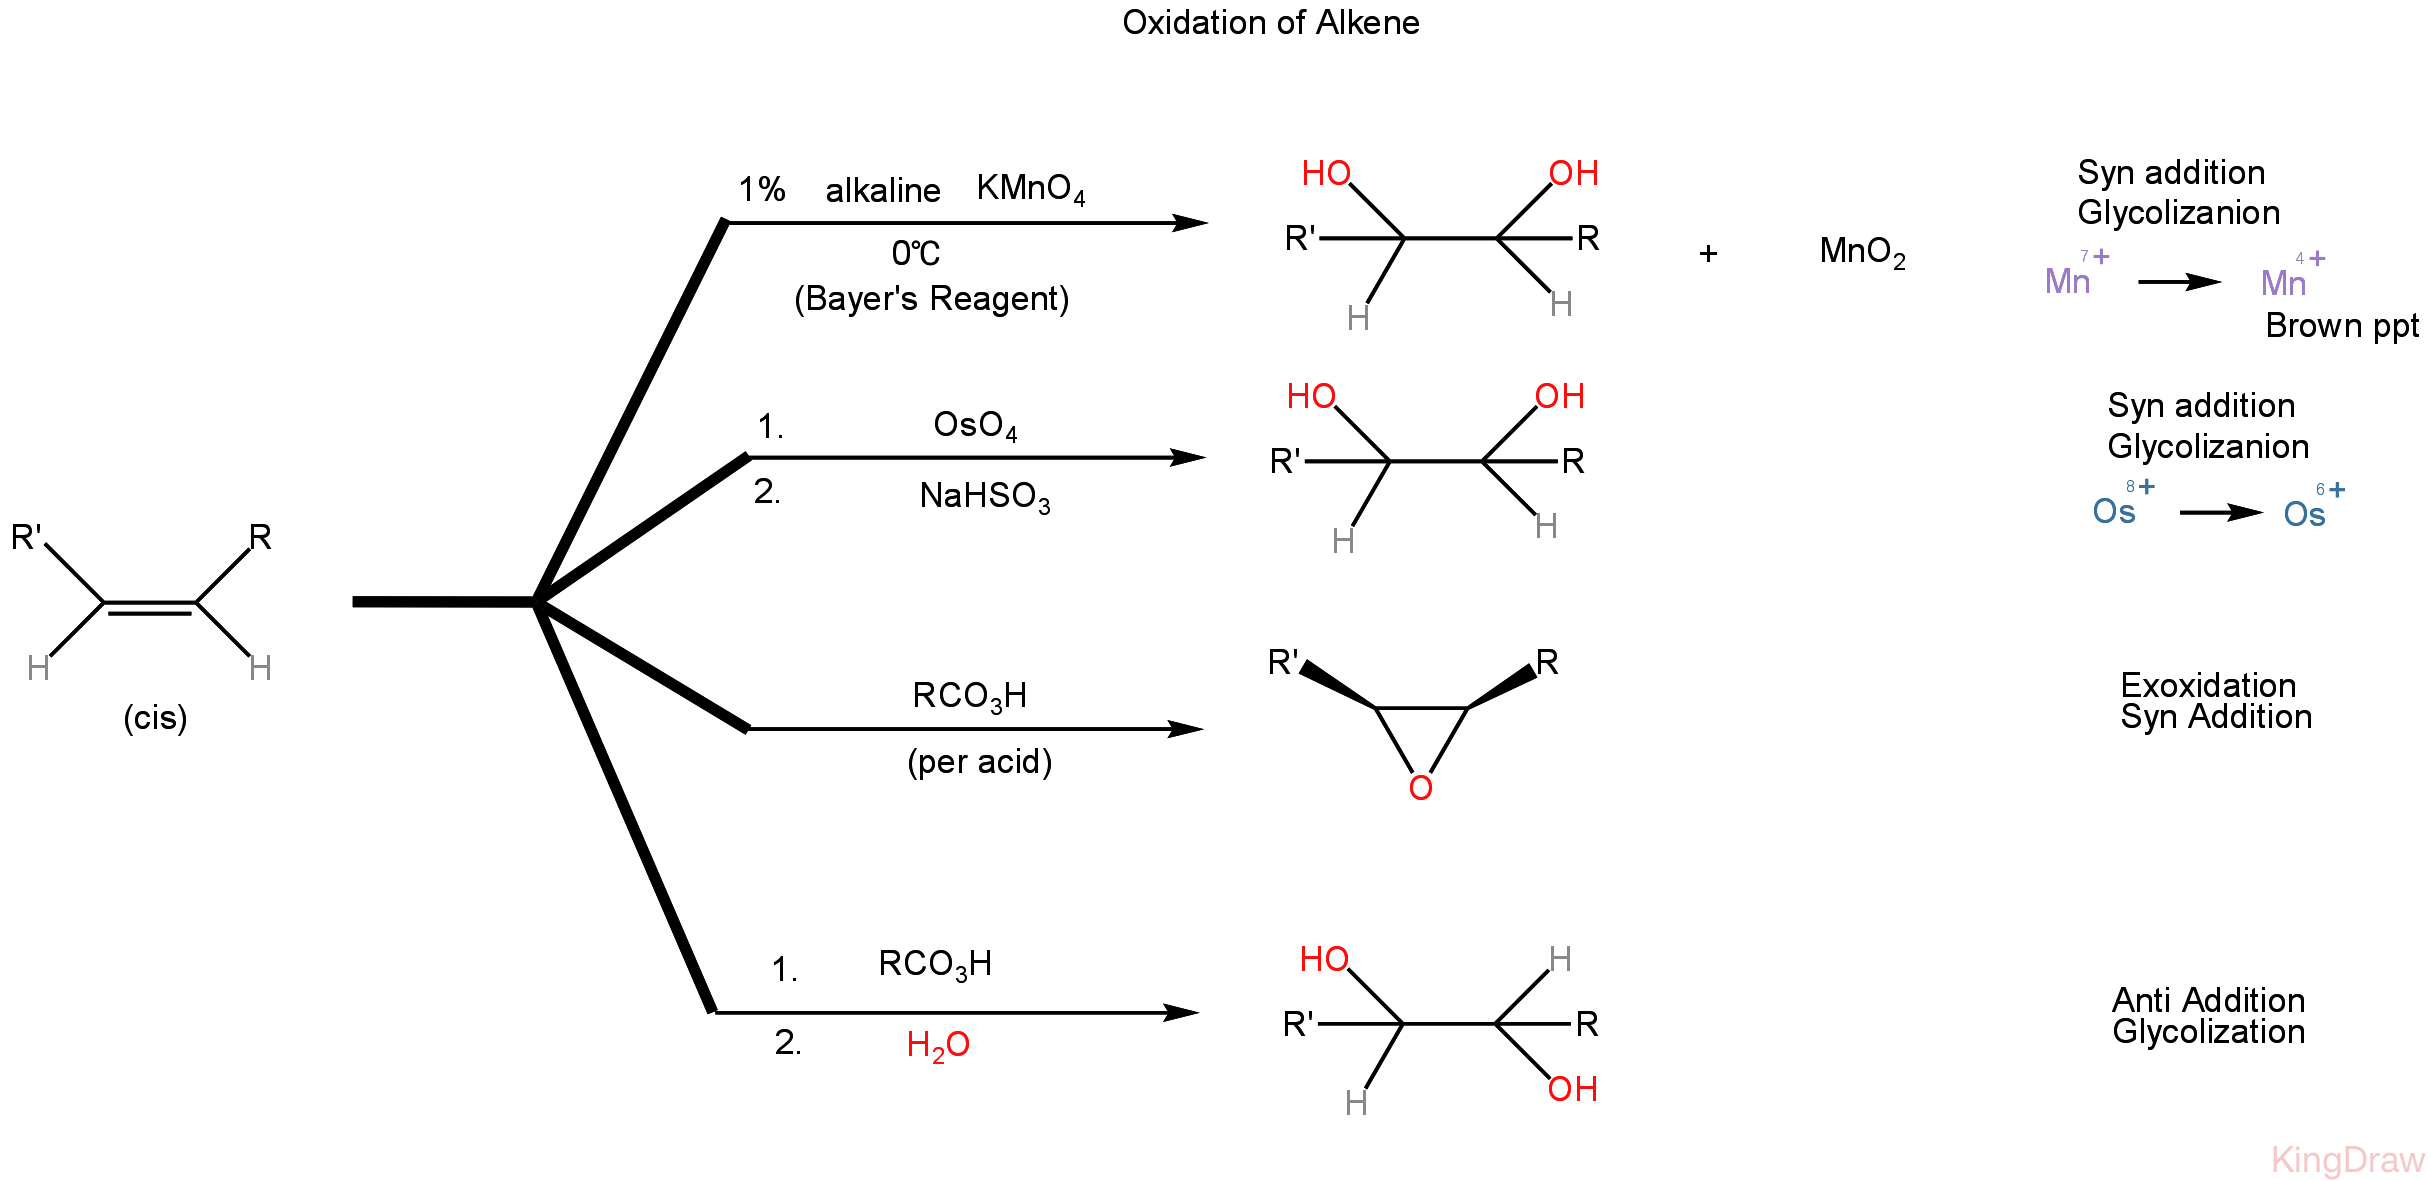
\includegraphics[scale=0.18]{oxidationofalkene_1723137821943.PNG}

\section{Soda Lime Decarboxylation}
\subsection{Reaction and Mechanism}
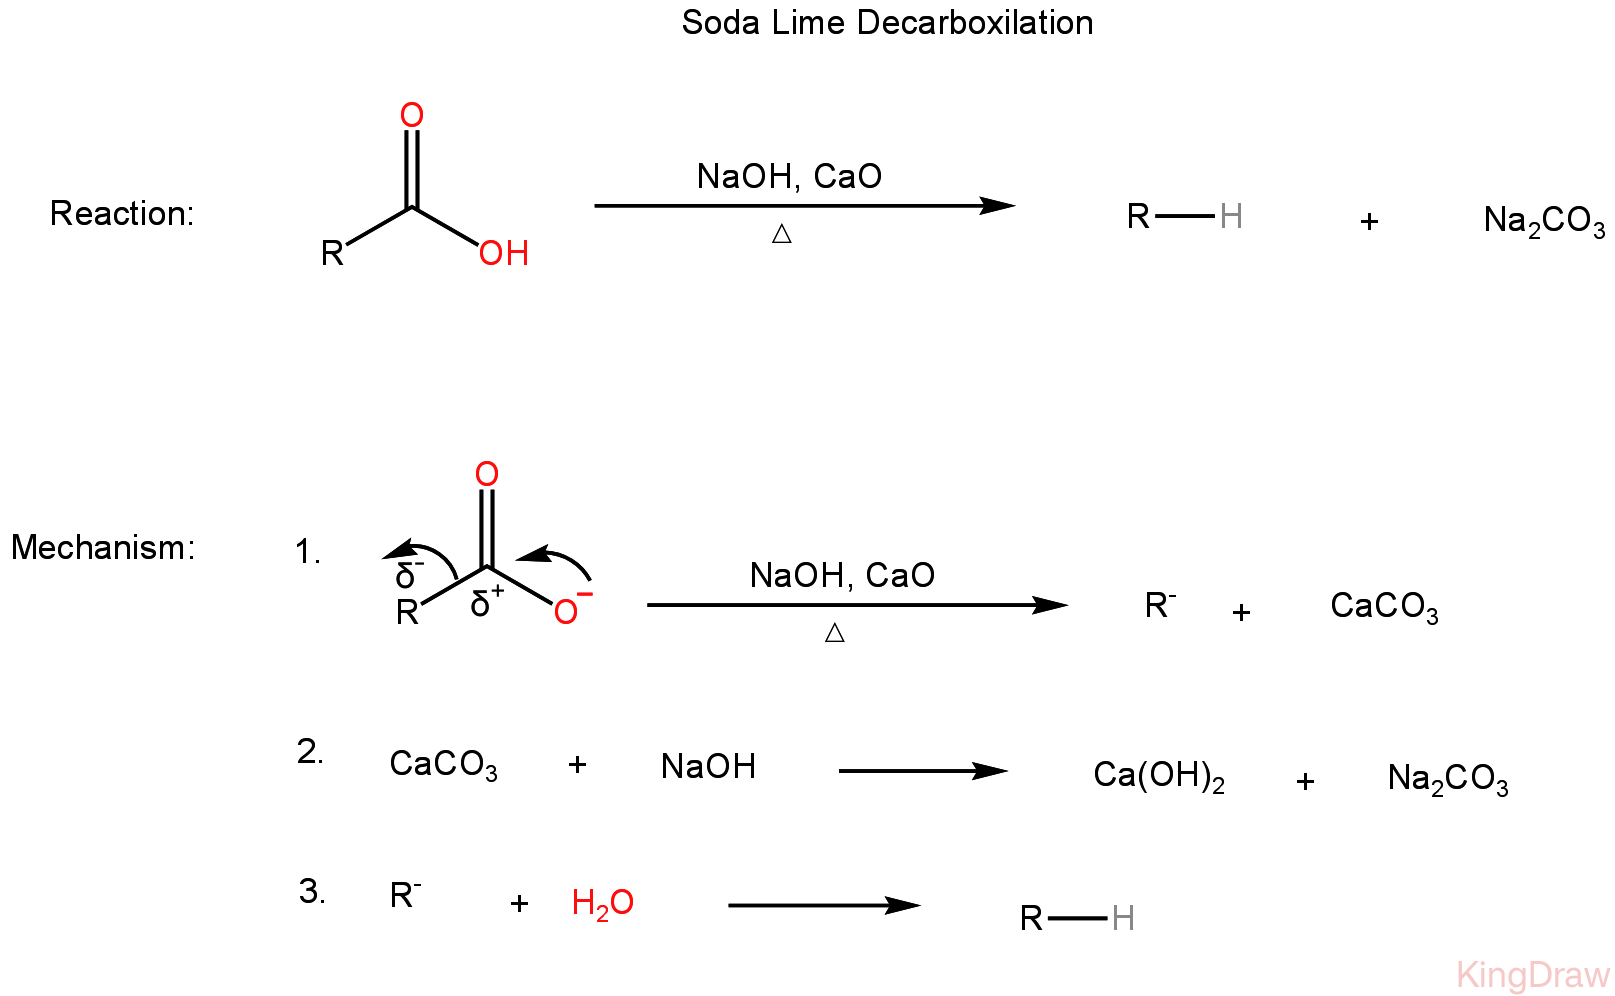
\includegraphics[scale=0.25]{Sodalime_1723140982114.PNG}
\subsection{Reaction Observations}
\begin{enumerate}[i.]
    \item $3:1$ of $NaOH$ and $CaO$ taken respectively.
    \item $C^-$ obtaied as intermediate.
    \item $ROR \propto \textit{ Stability of } C^-$
    \item a.k.a Oakwood Degradation
\end{enumerate}

\section{Ozonolysis}
\subsection{Reaction and Mechanism}
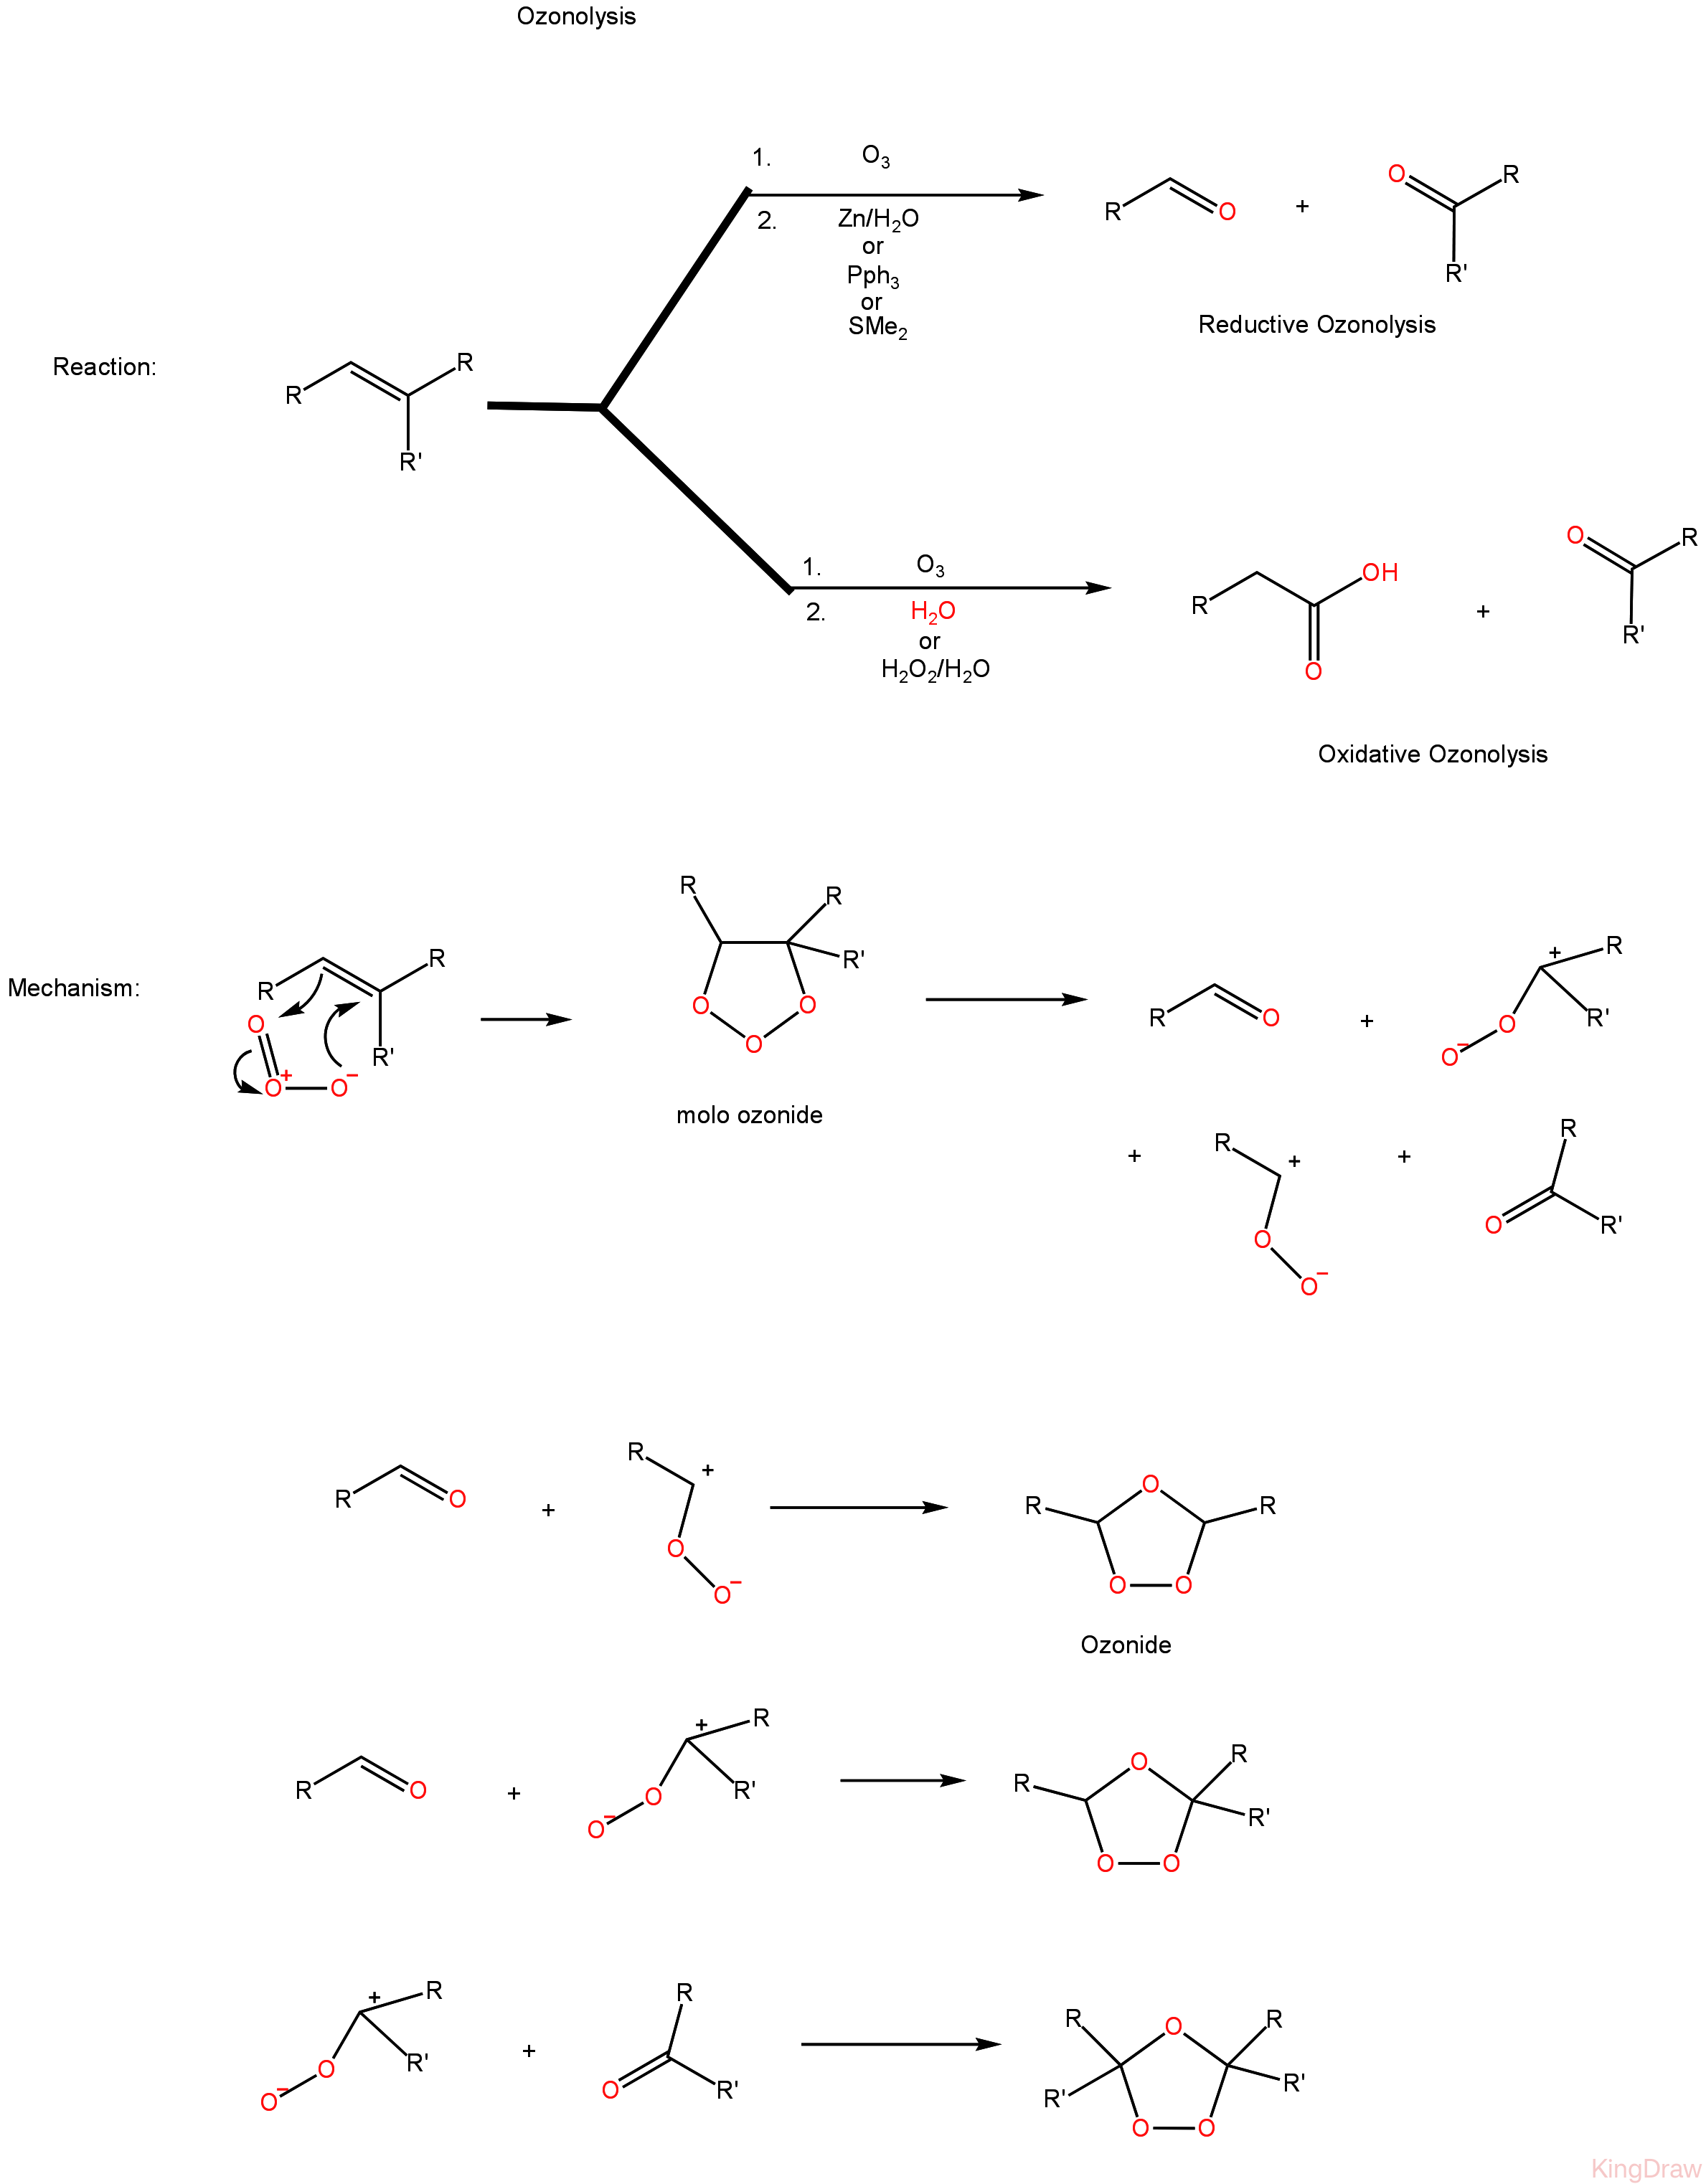
\includegraphics[scale=0.159]{ozono_1723144362447.PNG}
\section{Reactions of Hot $KMnO_{4}$}
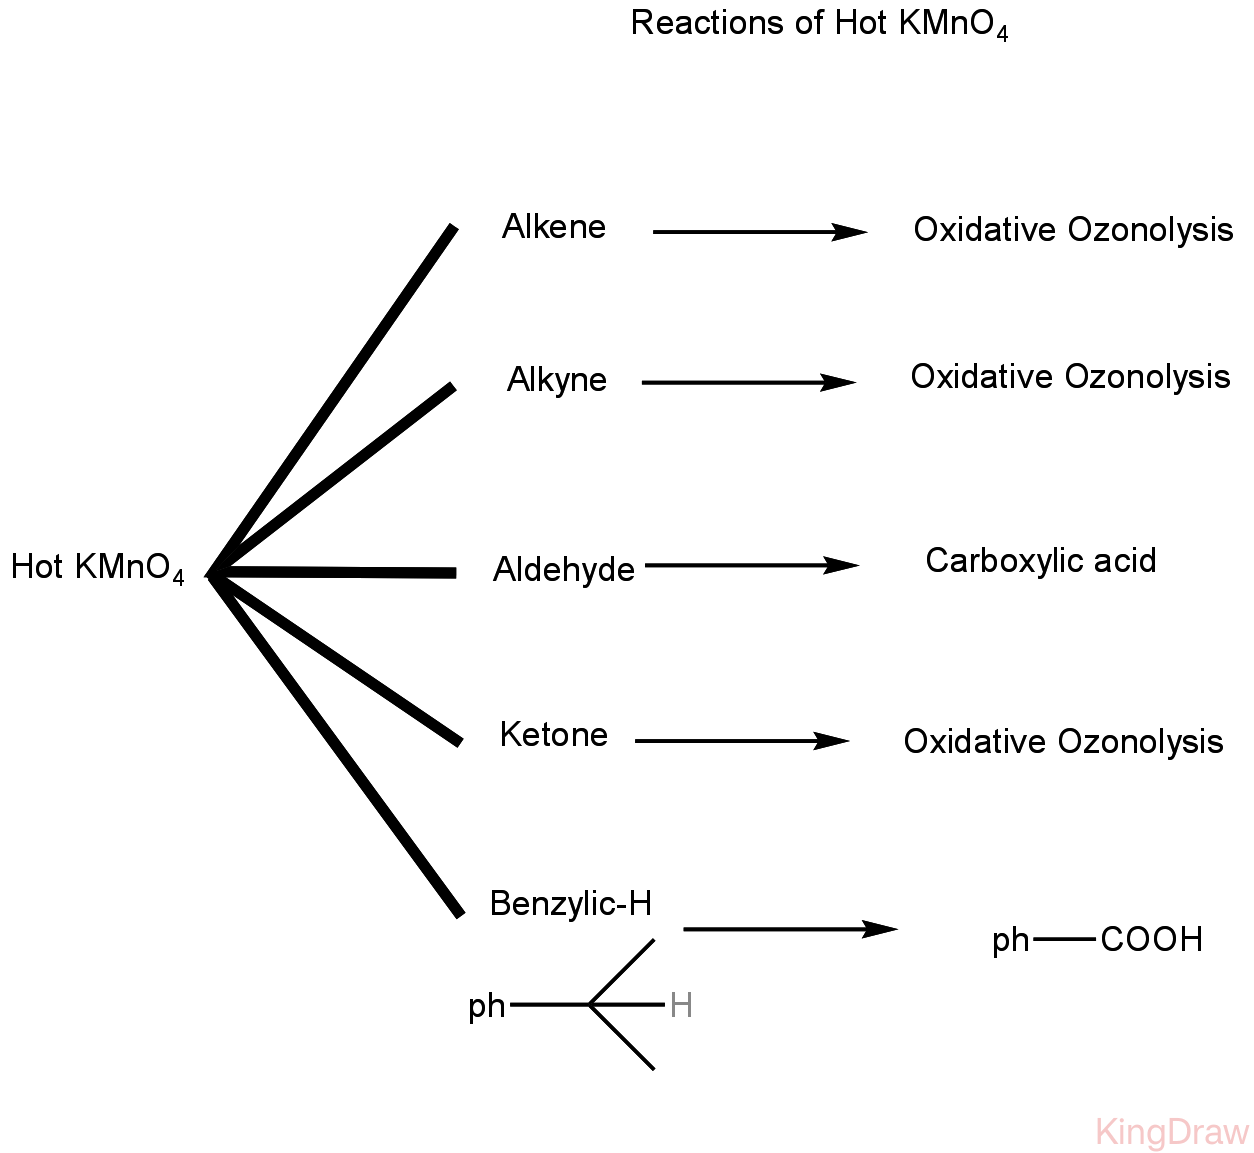
\includegraphics[scale=0.25]{rxofhotKMnO4_1723157430331.PNG}

\begin{enumerate}[i.]
    \item If Benzylic $\prescript{12}{6}{C}$ has any $-H, = , \equiv$ present then it will convert to benzoic acid.
    \item If there are multiple rings present in a compound, then the ring with more electron density will oxidize first.
\end{enumerate}
\section{Hydrolysis of Carbides}
\begin{enumerate}[i.]
    \item Hydrolysis of a Carbide results in formation of a Hydrocarbon and Hydroxide.
    \item Hydrolysis is a non redox reaction,\\
          Hence, $$\textit{oxidation state of $\prescript{12}{6}{C}$ in carbide $=$ oxidation state of $\prescript{12}{6}{C}$ in hydrocarbon.}$$
          $$\textit{Oxidation state of Metal in Carbide = Oxidation of metal in Hydroxide}$$
    \item The suffix $-ide$ in Carbide indicates that oxidation state of $\prescript{12}{6}{C} <0$ i.e. it is an anion.
\end{enumerate}
\section{Aromatization Reactions}
\subsection{Reaction of Alkyne inside Red Hot $Fe$ Tube}
$$on hold$$
\section{Electrophilic Aromatic Substitution}
\subsection{Reaction and Mechanism}
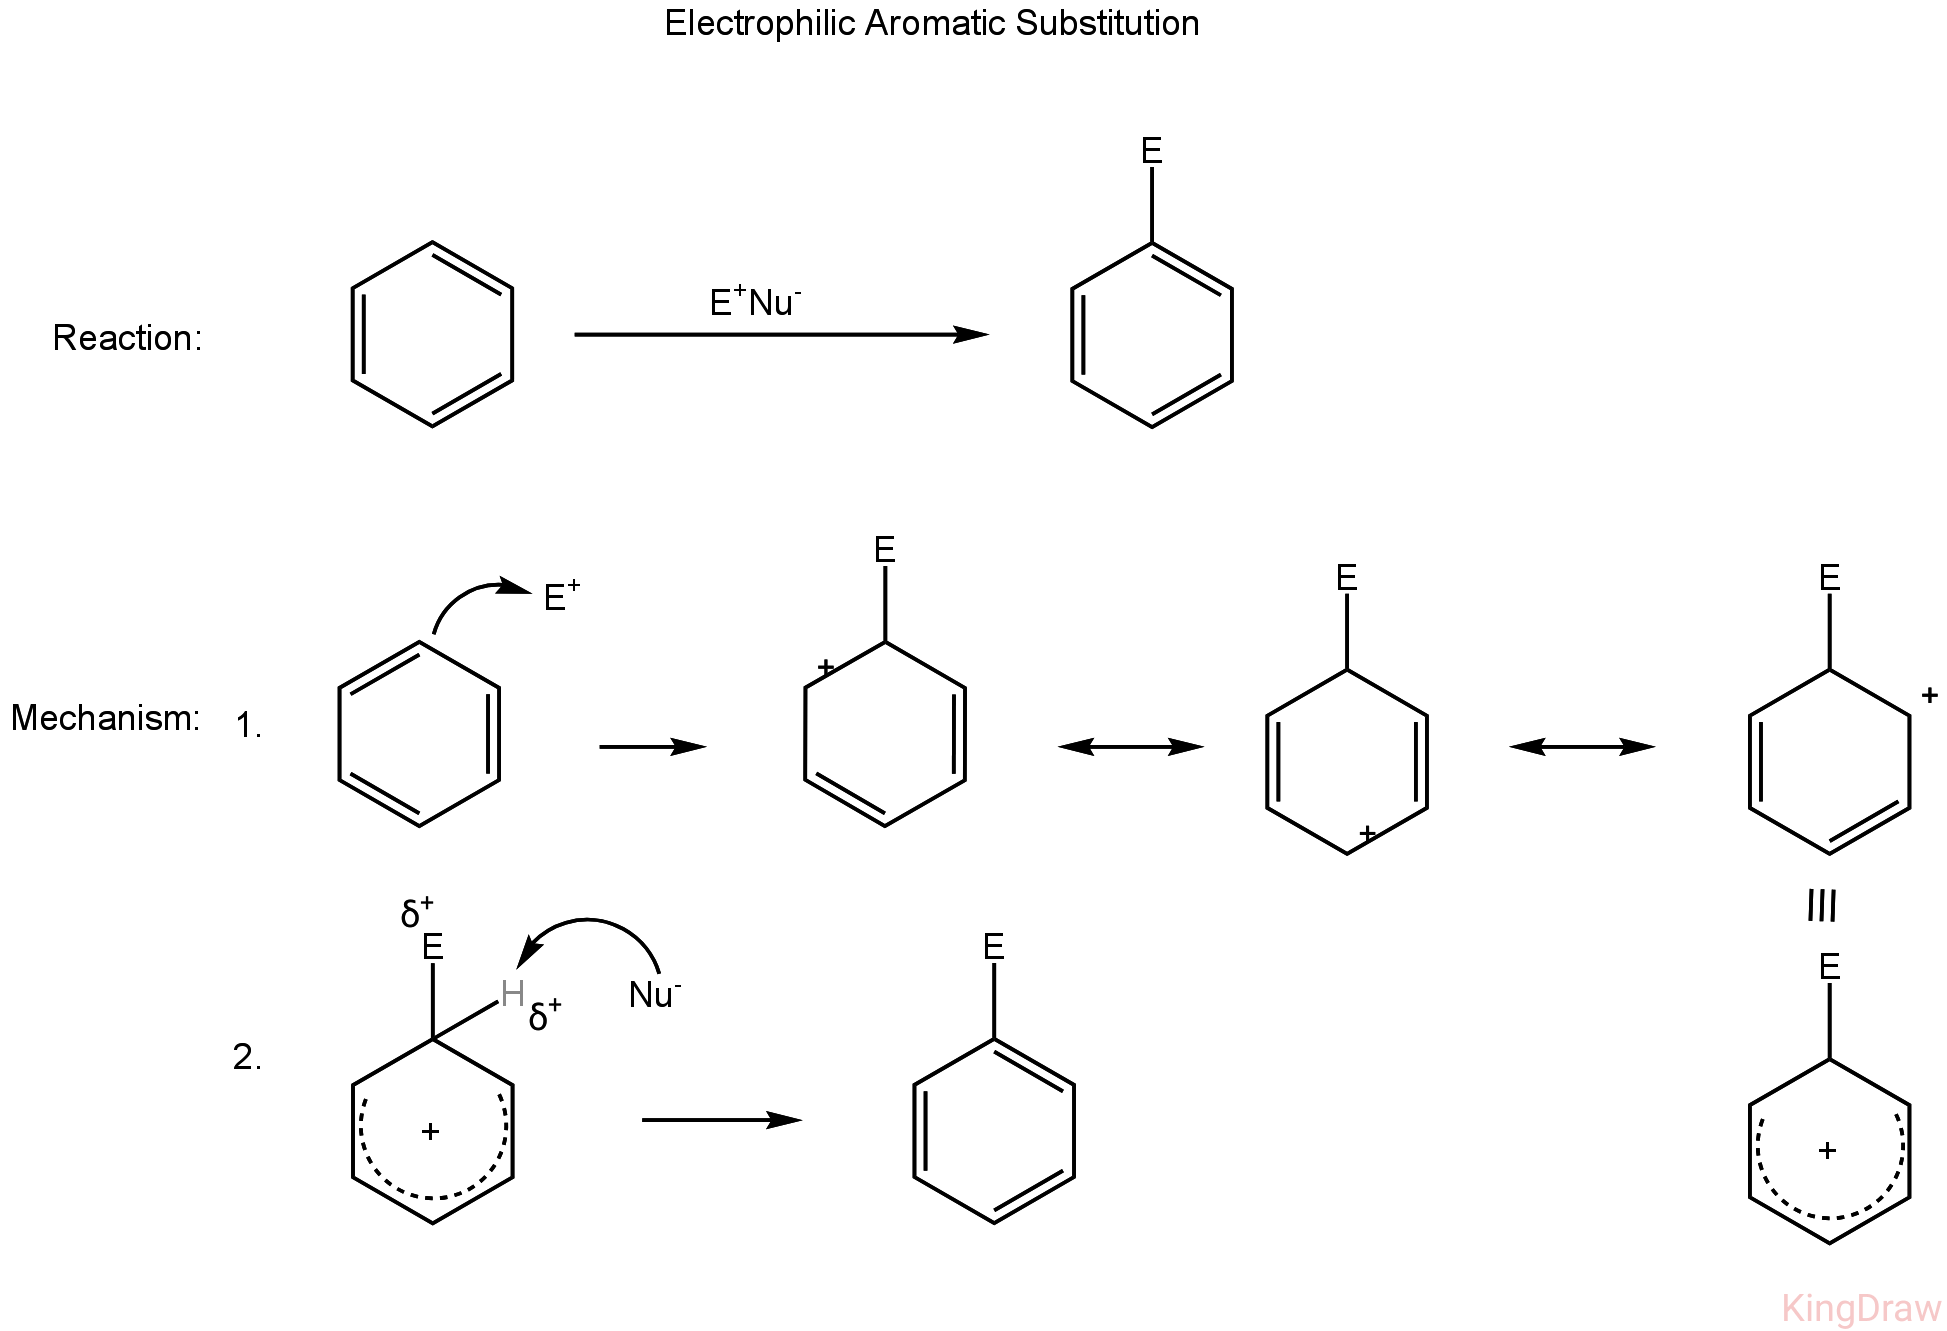
\includegraphics[scale=0.23]{EAS_1723190078116.PNG}
\subsection{Reaction Observations}
\begin{enumerate}[i.]
    \item $\sigma$ complex obtaied as intermediate.
    \item Formation of arenium ion is RDS.
    \item Rate law, $ROR=k [Ar-H][E^+]$
    \item Bimolecular Reaction
    \item $ROR \propto \textit{ Stability of  } C^+$
    \item EDG will increase the rate.
    \item Reaction can be reversible and irreversible.
\end{enumerate}
\subsection{Reversiblity of EAS}
EAS can be Reversible if,
\begin{itemize}
    \item $E^+$ is very stable [Alkylation (tert-Butyl cation), Iodination ($I^+$)]
    \item $E$ is gasous [Sulphonation ($SO_{3}$), Carboxylation ($CO_{2}$), Azotization ($N_{2}$), etc.]
\end{itemize}
\subsection{Reativity and Orientation}
\begin{itemize}
    \item Reacitvity is decided by net effect of $E$.
    \item Orientation is decided by stability of $\sigma$ complex.
    \item Reactivity, $EDG>Robinhood>EWG$
    \item EDG are $o,p$ directing.
    \item EWG are $m$ directing.
    \item Robinhood are $o,p$ directing.
\end{itemize}
\end{document}